\documentclass[11pt,a4paper]{book}
% \usepackage{titlesec}
\usepackage[legalpaper, margin=0.8in]{geometry}
\usepackage[brazil]{babel}
\usepackage[utf8]{inputenc}
\usepackage{xcolor}
\usepackage{listings}
\usepackage{amsmath}
\usepackage{amssymb}
\usepackage{amsfonts}
\usepackage{graphicx}
\usepackage{titling}
\usepackage{caption}
\usepackage[colorlinks=true,linkcolor=blue!80!brown!80!red]{hyperref}
\renewcommand{\thechapter}{\Roman{chapter}}
\renewcommand{\thesection}{\arabic{chapter}.\arabic{section}}
\renewcommand{\mod}[1]{\;\left(\bmod\; #1\right)}
\newcommand\tab[1][0.5cm]{\hspace*{#1}}
\usepackage{tocloft}

\addtolength{\cftchapnumwidth}{15pt}


\definecolor{mygreen}{rgb}{0.1,0.1,1.0}
\definecolor{mygray}{rgb}{0.5,0.5,0.5}
\definecolor{mymauve}{rgb}{0.58,0,0.82}
\lstset{ 
  backgroundcolor=\color{white},   % choose the background color; you must add \usepackage{color} or \usepackage{xcolor}; should come as last argument
  basicstyle=\ttfamily,        % the size of the fonts that are used for the code
  breakatwhitespace=false,         % sets if automatic breaks should only happen at whitespace
  breaklines=true,                 % sets automatic line breaking
  captionpos=b,                    % sets the caption-position to bottom
  commentstyle=\color{mygreen},    % comment style
  deletekeywords={...},            % if you want to delete keywords from the given language
  escapeinside={\%*}{*)},          % if you want to add LaTeX within your code
  extendedchars=false,              % lets you use non-ASCII characters; for 8-bits encodings only, does not work with UTF-8
  firstnumber=1,                % start line enumeration with line 1000
  frame=single,	                   % adds a frame around the code
  keepspaces=true,                 % keeps spaces in text, useful for keeping indentation of code (possibly needs columns=flexible)
  keywordstyle=\color{blue},       % keyword style
  language=C++,                 % the language of the code
  morekeywords={*,...},            % if you want to add more keywords to the set
  numbers=left,                    % where to put the line-numbers; possible values are (none, left, right)
  numbersep=5pt,                   % how far the line-numbers are from the code
  numberstyle=\tiny\color{mygray}, % the style that is used for the line-numbers
  rulecolor=\color{black},         % if not set, the frame-color may be changed on line-breaks within not-black text (e.g. comments (green here))
  showspaces=false,                % show spaces everywhere adding particular underscores; it overrides 'showstringspaces'
  showstringspaces=false,          % underline spaces within strings only
  showtabs=false,                  % show tabs within strings adding particular underscores
  stepnumber=1,                    % the step between two line-numbers. If it's 1, each line will be numbered
  stringstyle=\color{mymauve},     % string literal style
  tabsize=2,	                   % sets default tabsize to 2 spaces \lstinputlisting; also try caption instead of title
}
% \title{Monkeys LIB 2.0\\ Guadalajara Edition}

% \subtitle{Guadalajara Edition}
\author{Monkeys}
\date{2024}

\begin{document}
\begin{titlingpage} %This starts the title page
\begin{center}

\includegraphics[width=5cm]{t8.png}\\ %Put the logo you want here
\vspace{8cm} %You can control the vertical distance
\begin{huge} 
\textbf{Monkeys LIB 3.5} \\
\theauthor\\
\end{huge}
\vspace{12cm} %Put the distance you need.

\includegraphics[width=5cm]{UFG_LOGO.png}\\ %Put the logo you want here
\begin{LARGE}
\thedate
\end{LARGE}
\end{center}
\end{titlingpage}
 
 % https://www.overleaf.com/7646931546nfyjyscbbjjm
{\fontsize{40}{48} \selectfont }
\tableofcontents{}
 \chapter{Begin}
    \section{Who did this}
    Sometimes saying thank you is important, this book have the name and the heart of a group, full of disagreements. We are \textbf{different} and that is what makes us \textbf{strong}. Believe in yourself, and when u can't, believe in the people which are in your side.

    Thank you.

    Here is a list of names which contributed to build this book (for those who are asking, it was sorted by random\_shuffle  in C++20 using srand(252)):
    \begin{itemize}
        \item Lesin
        \item Alunea
        \item Nopebi Lifesa
        \item Atak Kichan
        \item Faslecar
        \item Nollyad
        \item Laelovatsug
        \item Ognol Tohberum
        \item Nhotivew
    \end{itemize}
    \section{tips}
    \begin{itemize}
    \item Remember that binary lifting isn't just for trees.
    
    \item Expected value? contribution is the way.
    
    \item DP? maybe a slow solution can be optimized.
    
    \item Chill, the contest is long, starting slow is good...
    
    \item Breath, drink water, make jokes, eat chocolate, at the end, have fun with your friends.
    
    \item A Greedy is a risk, but can be done. No one knows how to proof this shit anyway...
    \item flow? is this bipartite?
    \item remember what u can do in bipartite graphs:
    \begin{itemize}
        \item minimum vertex cover = maximum matching
        \item clique maximum(same as previous one) 
        \item maximum independent set = complement of minimum vertex cover
    \end{itemize}
    
    \item Remember, a binary search can simplify a lot!

    \item Can you model any recurrence?

    \item Write alot, Think out, Text.

    \item Don't be fixed in finding a fast solution, find one solution, and then, try to understand it.

    \item are there modulus? maybe splitting in cases can help.

    \item is this monotonic(increasing or decreasing)?
    
    \item Geometry has 4 options: Line sweep, binary search, Convex hull and Math.

    \item Game theory? just brute. recurrence in big num? just brute. Overall bruting is gud.
    
    \item BREATH!
    
    \item Your friends are here to help!!!
    
    \item Hug each other, spread love, not war.
    
    \item A funny joke doesn't have to offend a friend.
    
    \item YOU ARE A TEAM!!!

    \item idk maybe guessing that only checking primes is enough(if it doesn't work, try with powers of two)

    \item if u can't do $n \log$, just do $n\log^2$ u bitch
    
    \item remember, you can do some factorial stuff using convolutions.
    
    \end{itemize}
    
    % \newpage

    % \section{coisas pra fazer na lib}

    % \begin{itemize}
    %     \item Padronizar os códigos de geometria;
    %     \item Fazer o BigInt com Karatsuba;
    %     \item Convolução de Teoria dos Números;
    %     \item Colocar a nova Treap;
    % \end{itemize}

    \newpage
    \section{template - makefile - terminaltricks}
    \lstinputlisting{./solutions/template.cpp} 

    \lstinputlisting{./solutions/makefile}
    \lstinputlisting{./solutions/terminaltrick} 
    \newpage
    \section{math formulas}
    \begin{itemize}
        \item $a_n = a_{n-1} + r$
        \item $a_n = a_1 + (n-1)*r$
        \item \begin{Large}
            $soma_{(l,r)} = \frac{(a_l + a_r) * (r-l+1)}{2}$
        \end{Large}
    \end{itemize}

    \begin{itemize}
    \item $a_n = a_{n-1}*q$
    \item $a_n = a_1*q^{n-1}$
    \item \begin{Large}
            $soma_{(l,r)} = \frac{a_l  * (q^{(r-l+1)}-1)}{q-1}$
        \end{Large}
    \end{itemize}
     
    \textit{Fórmula de Heron para Triângulos:} $\sqrt{p\cdot (p-b) \cdot (p-c) \cdot (p-d)}$
    
    \textit{Fórmula de Heron para Quadriláteros:}
    
    \begin{itemize}
        \item $p = (a+b+c+d)/2$
        \item $A = \sqrt{(p-a) \cdot (p-b) \cdot (p-c) \cdot (p-d)}$
        \item $A \rightarrow$ Maior área formada por 4 lados de um quadrilátero.
    \end{itemize}
    
    
    \begin{figure}[ht]
    \begin{center}
    \begin{minipage}{.48\textwidth}
        \centering
        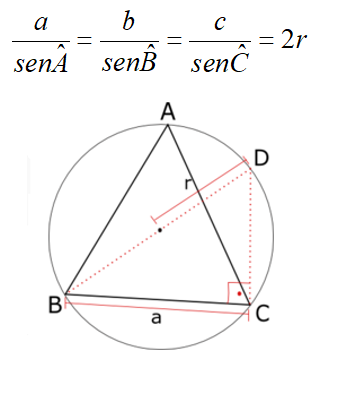
\includegraphics[scale=0.7]{imgs/leidossenos.png}
        \captionof{figure}{Lei dos senos}
    \end{minipage}
    \begin{minipage}{.48\textwidth}
    \centering
        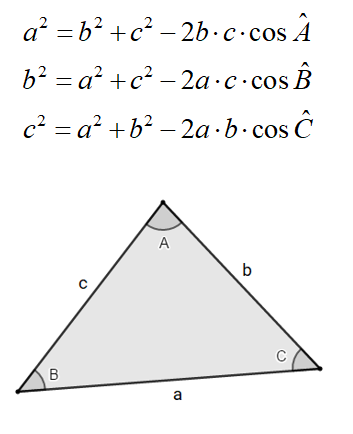
\includegraphics[scale=0.7]{imgs/leidoscosenos.png}
        \captionof{figure}{Lei dos cossenos}
    \end{minipage}
    \end{center}
    \end{figure}
    \section{Stress Test}
    During the contest, sometimes u will need to stress test an solution.
    the steps are:
    \begin{itemize}
        \item Code a Brute Force(do as lazy as possible, focus in not spend time coding it)
        \item Code a generator (in the following lines there are some generators for vectors, trees and graphs)
        \item run the stress test.
        \item To use this thing, just run "bash s.sh" and see everything working!
    \end{itemize}

    The run part will have some bash function like this:
    
    \lstinputlisting{./solutions/stress.sh}

    \subsection{Vector Generator}

    Simple vector generator (just for remembering).

    Has two parameters, the quantity of elements the the biggest element.
    
    \lstinputlisting{./solutions/gen.cpp}
    
    \subsection{Tree Generator}
    The following code generates good trees.
    It has two parameter, the quantity of vertices and the id of the test(used for generation).

    \lstinputlisting{./solutions/gen_tree.cpp}

    
 \chapter{Algebra}
    
    \section{Inteiro Modular}
    Classe para lidar com problemas relacionados a operações modulares.
    
    \lstinputlisting{./solutions/Algebra/modint.cpp}
    \section{Matrix Power}
    \subsection{Graph Paths I}
    Consider a directed graph that has $n$ nodes and $m$ edges. Your task is to count the number of paths from node $1$ to node $n$ with exactly $k$ edges.
    \lstinputlisting{./solutions/Algebra/GraphPathsI.cpp}
    
    \subsection{Graph Paths II}
    Consider a directed weighted graph having $n$ nodes and $m$ edges. Your task is to calculate the minimum path length from node $1$ to node $n$ with exactly $k$ edges.
    \lstinputlisting{./solutions/Algebra/GraphPathsII.cpp}
    \section{FFT}
    \subsection{Simple FFT}
    Multiplicação de dois polinômios em tempo $O((n+m) \cdot \log(n+m))$
    O polinômio $ a + bx + cx^2 + dx^3$ é representado na forma de vetor como $[a, b, c, d]$.
    Para usar a função $multiply$, crie dois vectors $vector<int> a, b;$ apos fazer $multiply(a, b);$ tem-se o vector polinômio com os coeficientes da multiplicação de a e b.
    \lstinputlisting{./solutions/Algebra/fft.cpp}
    \subsection{FFT To solve String with Wildcards}
    Given two strings $s$ and $t$, with $t$ having wildcards that can match with any character, returns the number of ocurrence of $t$ in $s$.
    Solution $O(nlogn)$.
    \bigskip
    (Original Problem: Maraton Nacional de Programacion Colombia 2016 - Wildcards).
    \lstinputlisting{./solutions/Algebra/fft_wild_card.cpp}
    \subsection{FFT modular (NTT)}
    To use a modular FFT, also known as NTT, you need a $n$-th root of ur modulus and then define some values in general u can say :
    
    $mod = x*2^k$
    
    $G = 3 $ or $5$
    
    $root = G^{mod/(2^k)}$
    
    $root_1 = root^{-1}$
    
    $root_{pw} = 2^k$
    \lstinputlisting{./solutions/Algebra/ntt.cpp}

    \subsection{FWHT (fft using xor/and/or)}
    FFT but the expoent operation is xor/and/or.

    There are some crazy problems where u need to multiply $N$ polynomials of the form $x^0 + x^i$ and the $i$ can be up to $N$. the main approach is to use some D\&C to multiply those and to keep the polynomials divide in two parts. It is also coded down here. Operations can be modular.
    \lstinputlisting{./solutions/Algebra/FWHT.cpp}
    \section{Gauss}
    \subsection{Markov Chains}
    if we have $E(i) = 1 + \sum_{j=0}^{N-1} P[i][j] * E(j)$

    We can model as a System of linear equations of the form:

    $E(i) - \sum_{j=0}^{N-1} P[i][j] * E(j) = 1$

    So:

    \[ \begin{bmatrix}
         1-P[0][0] & -P[0][1] & \cdots & -P[0][N-1]\\
         -P[1][0] & 1-P[1][1] & \cdots & -P[1][N-1]\\
         \vdots & \vdots & \ddots & \vdots\\ 
         -P[N-1][0] & -P[N-1][1] & \cdots & 1-P[N-1][N-1]\\
     \end{bmatrix}
     \times
     \begin{bmatrix}
         E(0)\\
         E(1)\\ 
         \vdots\\ 
         E(N-1) 
     \end{bmatrix}
      =
     \begin{bmatrix}
         1\\
         1\\ 
         \vdots\\ 
         1 
     \end{bmatrix} \]


    Works with probabilities as well, but without the 1 in the sum.

    Gauss Solves a System of linear equations in $O(min(N,M)*N*M)$, with $N$ being the number of variables and $M$ being the number of equations.

    Given a Directed Graph, find the probability of a random path goes from $1$ to $300$ and does not step in $290 \cdots 299$
    \lstinputlisting{./solutions/Algebra/gauss.cpp}

    
    \subsection{Modular}
    Given a tree (undirected unweighted graph), assign for each node in this a color $c_i$ ($0 \leq c_i \leq k - 1)$, such that for each node $i$, $c_i$ is the sum of colors adjacents to $i$ mod $k$.
    \bigskip
    Compute the number of differents possible colorings.
    \bigskip
    Solution $O(n^3)$.
    \bigskip
    (Original Problem: LightOJ 1279 - Graph Coloring).
    \lstinputlisting{./solutions/Algebra/GaussModular.cpp}
    \subsection{Modular 2 (bitset)}
    Problem:
    
    a grid of switchs and each press in a switch i,j swaps the state of himself and the ones which are adjacent to it.
    
    If there is a way to make all on, print the switchs pressed.
    \lstinputlisting{./solutions/Algebra/gaussmod2.cpp}
    
    \subsection{Matrix rank}
    The rank of a matrix is the largest number of linearly independent rows/columns of the matrix. The rank is not only defined for square matrices.
    We can see that the other variables are "free", so can be uses to combinatorial problems.
    
    Example:
    
    Given a set of n integers, how many subsets have xor not equal to 0?
    \lstinputlisting{./solutions/Algebra/subset-nim.cpp}

    \subsection{Xor Basis}
    Cebolinha me mostrou essa parada, fazendo uma solução pro mesmo problema acima usando isso.

    Da pra gente saber se um X pertence ao XOR de algum subconjunto dos seus caras.

    o total de caras q pertence ao subconjunto é $2^{B.size()}$.

    \lstinputlisting{./solutions/Algebra/xorbasis.cpp}
    
    \section{Chinese Remainder Theorem}

    % \subsection{Coprimes congruences}
    % Given a list $A$, and a list $M$, find a $X$ that $X = A_i mod M_i$. $X$ is given $mod LCM(M_1,\cdots, M_{n-1})$.
    % \lstinputlisting{./solutions/Algebra/crt.cpp}

    \subsection{Algorithm}

    Given $(a, n, b, m)$, find a $X$ such that $X = a \mod n$ and $X = b \mod m$. $X$ is given mod LCM$(n, m)$.
    \lstinputlisting{./solutions/Algebra/crt2.cpp}

    \subsection{Lucas Theorem}

    Given $n, k$ and $m$, find $\binom{n}{k}$ mod $m$, where $(n, k \le 10^{9})$, $m$ is a square-free number less than or equal to $10^{9}$ and each prime that appears on $m$ is less than $50$. A Square-Free number is a number that, in his prime factorization, each prime appears exactly once.

    \lstinputlisting{./solutions/Algebra/Lucas.cpp}
    
    \section{Simplex}
    Maximize ${\textstyle \mathbf {c^{T}} \mathbf {x} }$
subject to ${\displaystyle A\mathbf {x} \leq \mathbf {b} }$ and ${\displaystyle \mathbf {x} \geq 0}$
    \lstinputlisting{./solutions/Algebra/simplex.cpp}
    \section{GCD Array Trick}
    Way to store all gcds in a array range . For each $i$ you store every different gcd sub-segment that exists starting at $i$.
    
    In this problem you need to find a $Max(gcd(A[l],\cdots,A[r])*(r-l+1))$.
    \lstinputlisting{./solutions/Algebra/gcdrobado.cpp}
    \section{Implementation of Polynomials}
    Algorithm to find a root, and also to divide a poly by some (x+c).
    \lstinputlisting{./solutions/Algebra/polynomials.cpp}
    \section{Combinatorial}
    Multiple combinatorial solutions.
    
    Number of ways to take $K$ objects, between $N -> Comb(N,K)$
    
    Number of ways to put $N$ objects in $K$ boxes (stars and bars) $-> sb(N,K)$

    Count how to label $N + K$ pairs of parentheses with $K$ $'('$s already fixed $-> catalan(N,K)$
    
    \lstinputlisting{./solutions/Algebra/combinatorial.cpp}
    Version that Sabino likes
    \lstinputlisting{./solutions/Algebra/comb.cpp}
    \subsection{Derangements}
    The number of derangements of $n$ numbers, expressed as $!n$, is the number of
    permutations such that no element appears in its original position. Informally,
    it is the number of ways $n$ hats can be returned to $n$ people such that no
    person recieves their own hat.
    
    Principle of Inclusion-Exclusion
    
    Suppose we had events $E_1, E_2, \dots, E_n$, where event $E_i$ corresponds to
    person $i$ recieving their own hat. We would like to calculate $n! - \lvert E_1 \cup E_2 \cup \dots \cup E_n \rvert$.
    
    We subtract from $n!$ the number of ways for each event to occur; that is,
    consider the quantity $n! - \lvert E_1 \rvert - \lvert E_2 \rvert - \dots - \lvert E_n \rvert$. This undercounts, as we are subtracting cases where more
    than one event occurs too many times. Specifically, for a permutation where at
    least two events occur, we undercount by one. Thus, add back the number of ways
    for two events to occur. We can continue this process for every size of subsets
    of indices. The expression is now of the form:
    
    $$n! - \lvert E_1 \cup E_2 \cup \dots \cup E_n \rvert = \sum_{k = 1}^n (-1)^k \cdot (\text{number of permutations with $k$ fixed points})$$
    
    For a set size of $k$, the number of permutations with at least $k$ indices can
    be computed by choosing a set of size $k$ that are fixed, and permuting the
    other indices. In mathematical terms:
    
    $${n \choose k}(n-k)! = \frac{n!}{k!(n-k)!}(n-k)! = \frac{n!}{k!}$$
    
    Thus, the problem now becomes computing
    
    $$n!\sum_{k=0}^n\frac{(-1)^k}{k!}$$
    
    which can be done in linear time.
    \section{Lagrange Interpolation}
    Suppose u have a polynomial of order $K$, and want to find $f(N)$, and N is really big.

    With Lagrange Interpolation, we can define any $f(x)$ as a linear combination of k+1 $f(u)$'s.

    The normal approach is to calc the first k+1 answers and use the to calculate $f(N)$.

    Math below:

    given the set of points .

    $l_j(x) = \frac{x-x_0}{x_j-x_0} * \cdots * \frac{x-x_{j-1}}{x_j-x_{j-1}} * \frac{x-x_{j+1}}{x_j-x_{j+1}} * \cdots * \frac{x-x_k}{x_j-x_k} $

    $f(x) = f(x_0)*l_0(x) + f(x_1)*l_1(x) + ... f(x_{k-1})*l_{k-1}(x) + f(x_k)*l_k(x) $
    
    \lstinputlisting{./solutions/Algebra/lagrange.cpp}
    Felipe Sabino, aka sabino1, version.
    \lstinputlisting{./solutions/Algebra/lagrangefelipe.cpp}
    % Teoria dos numeros vai ter uma seção propria
    \section{Discrete Log}

    \tab You have an modular equation with $a,b,x \in \mathbb{Z}$, you want to find a value for $x$
    
    $a^x \equiv b \;(\bmod\; m)$

    If you only want to find a solution, you just have to consider values between $[0,m-1]$ because, by the Pigeonhole Principle, $a^0,a^1,\dots,a^m$ you can only have m possible values, so minimally $a^m$ it's going to be a value that already appeared and it's going to cycle. So you have to consider values between $[0,m-1]$.

    However, the values of $m$ can be big, $1e9$, there's a way to solve it in $s\sqrt{m}$, the Baby-step giant-step.

    Let's consider that $gcd(a,m) = 1$ and rewrite the expression (remember you can write every integer with $x = q*p + r$, where $0 \leq r < p$, and with that you can also write $x = (q+1)*p -r$, where $0 \leq r < p$):

    $$
    a^x \equiv b \mod{m} 
    $$
    $$
    a^{q*p-r} \equiv b \mod{m}
    $$
    $$
    a^{q*p}*a^{-r} \equiv b \mod{m}
    $$
    $$
    a^{q*p} \equiv b*a^r \mod{m}
    $$

    If you determine a good value for $p$, you can decrease the range of possible values of both $q$ and $r$, let $p = \sqrt{m}$, then $0 \leq p \leq \sqrt{m}+1$ (the plus 1 comes from the minus from the $r$) and $0 \leq r < \sqrt{m}$, so you can precalculate the values of $a^{q*p}$ for all $0 \leq p \leq \sqrt{m}$ and $b*a^{r}$ for all $0 \leq r < \sqrt{m}$, so in the end you have $O(\sqrt{m})$. And to find values of $q$ and $r$, you go through the values of $a^{q*p}$ and use binary search or two point to find a value $b*a^r$ that is equal.

    If $gcd(a,m) \neq 1$, then you can't calculate the inverse of $a^r$, however you can still try to solve it, let $g = gcd(a,m)$, if $g \nmid b$ then the equation doesn't have solution (if $g \mid a$ and $g \mid m$, then certainly, by linear combination, $g \mid b$). If $g \mid b$, then you can divide everyone by $g$. And do it until $gcd(a,m) \neq 1$. But after every time you do this operation you eliminate one $a$ from $a^x$.

    $$a^x \equiv b \mod{m}$$
    $$a^{x-1}*a \equiv b \mod{m}$$
    $$a^{x-1}*\frac{a}{g} \equiv \frac{b}{g} \mod{\frac{m}{g}}$$
    
    $$\dots$$
    
    $$a^{x-add}*\frac{a^{add}}{k} \equiv \frac{b}{k} \mod{\frac{m}{k}}$$

    After applying the operation $add$ times you have to solve the problem with new values where $gcd(a,\frac{m}{k}) \neq 1$.

    \lstinputlisting{./solutions/Algebra/discrete_log.cpp}    
        

    \section{Nelsi's anotations}
        \subsection{Kaplansky's Lemma} 
            \subsubsection{Lemma 1}
                Given a set of size $N$, how many subsets of size $K$ that do not contain consecutive elements exist?
                
                Basically, we will rewrite the elements of our set as $+$ and $-$. Such that between each pair of $+$, there is a $-$. Initially, we will choose $K$ plus signs. Then, we will have $x_1$ minus signs before the first plus, $x_2$ between the first and the second, and so on, up to $x_{\scriptscriptstyle K+1}$.
                \begin{align*}
                    x_1, x_{\scriptscriptstyle K+1} &\ge 0\\
                    x_i > 0 \; \forall \; 2 &\le i \le K 
                \end{align*}
        
                We have $N-K$ minus signs to distribute. Since $x_2$ to $x_{\scriptscriptstyle K}$ are positive integers, we will express $x_1$ and $x_{\scriptscriptstyle K+1}$ as positive integers in the form of $x'_1-1$ and $x'_{\scriptscriptstyle K+1}-1$, resulting in the equation:
                
                
                $x'_1 - 1 + x_2 + x_3 + ... + x_{\scriptscriptstyle K-1} + x_{\scriptscriptstyle K} + x'_{\scriptscriptstyle K+1}-1 = N-K$
        
                $x'_1 + x_2 + x_3 + ... + x_{\scriptscriptstyle K-1} + x_{\scriptscriptstyle K} + x'_{\scriptscriptstyle K+1} = N - K + 2$
        
                
                We know the formula for calculating how many integer solutions there are for a positive integer.
        
                $\binom{M-1}{P}$ Assuming $M$ is the desired answer and $P$ is the number of coefficients.
        
                In our problem, it takes the following form: $\binom{N-K+1}{K}$
    
            \subsubsection{Lemma 2}
            Given a circle with numbers from $1$ to $N$, in how many ways can we choose $K$ numbers without selecting neighboring ones?

            We can divide the problem into $2$ cases:

            If N belongs to the set, we need to choose $K-1$ elements from $N-3$ options. Following the previous lemma, our answer is:
            
            $\binom{N-K-1}{K-1}$
            
            
            If N does not belong to the set, we have to choose $K$ from $N-1$ options.Following the previous lemma, our answer is:
            
            $\binom{N-K}{K}$

            
            Summing up the two answers we obtained, we have:  $\binom{N-K-1}{K-1}\binom{N-K}{K}$ $=$ $\frac{N}{N-K}\binom{N-K}{K}$
        \subsection{Divisor Analysis - CSES} 
            \subsubsection{Number of Divisors}
                    Each divisor of the number can be written as $\prod_{i = 1}^N x_i^{\alpha_i}$
                    where $0 \leq \alpha_i \leq k_i$.
                    
                    Since there are $k_i + 1$ choices for $\alpha_i$, the number of divisors is
                    simply $\prod_{i = 1}^N (k_i + 1)$.
                    
                    We can calculate this by iterating through the prime factors in $\mathcal O(N)$
                    time.
                    
            \subsubsection{Sum of divisors}
            
                Let the sum of divisors when only considering the first $i$ prime factors be $S_i$. The answer will be $S_N$.
                
                $$\begin{aligned} S_i &= S_{i - 1} \sum_{j = 0}^{k_i} x_i^j\\ &= S_{i - 1} \cdot \frac{x_i^{k_i + 1} - 1}{x_i - 1}\\ \end{aligned}$$
                
                We can calculate each $S_i$ using fast exponentiation and modular inverses in
            $\mathcal O(N \log(\max(k_i)))$ time.
            
            \subsubsection{Product of divisors}

                Let the product and number of divisors when only considering the first $i$ prime
                factors be $P_i$ and $C_i$ respectively. The answer will be $P_N$.
                
                $$\begin{aligned} P_i &= P_{i - 1}^{k_i + 1} \left(x_i^{k_i(k_i + 1)/2} \right)^{C_{i - 1}} \end{aligned}$$
                
                Again, we can calculate each $P_i$ using fast exponentiation in
                $\mathcal O(N \log(\max(k_i)))$ time, but there's a catch! It might be tempting
                to use $C_{i - 1}$ from your previously-calculated values in part 1 of this
                problem, but those values will yield wrong answers.
                
                This is because $a^b \not \equiv a^{b \bmod p} \pmod{p}$ in general. However, by
                Fermat's little theorem, $a^b \equiv a^{b \bmod (p - 1)} \pmod{p}$ for prime
                $p$, so we can just store $C_i$ modulo $10^9 + 6$ to calculate $P_i$.

        \subsection{Bracket Sequences II - CSES}
            For the "Bracket Sequences II" solution, we will first calculate the factorials and perform the following checks. Initially, we will check if the bracket sequence (BS) becomes irregular at any point; if it does, we return $0$. Additionally, we will verify if our right bracket sequence (RBS) has all $N$ elements; if it does, we return $1$.

            After these base case checks, we will proceed to calculate the Catalan number for this value.
 
            The standard formula for the Catalan number is: \\

            $C_n = \binom{2n}{n} - \binom{2n}{n - 1}$

            This formula means that out of the $2n$ opening parentheses, we will choose $n - 1$ to close. We will make a small modification to it. We will keep track of the number of parentheses that have already been opened and closed and substitute that into the formula. \\

            $C_n = \frac{2n - (open + close)}{(n-open)!(n-close)!} - \frac{2n - (open + close)}{(n-open-1)!(n-close+1)!}$


        
    \section{Multiplicative Functions}
   In number theory, a multiplicative function is an arithmetic function $f(n)$ of a positive integer $n$ with the property that $f(1) = 1$ and

$$\displaystyle f(ab)=f(a)f(b)$$

whenever a and b are coprime.

    Examples of multiplicative functions:
    \begin{itemize}
        \item $gcd(n,k)$: the greatest common divisor of n and k, as a function of n, where k is a fixed integer.
\item {$\displaystyle \varphi (n)$}: Euler's totient function 
{$\displaystyle \varphi$ }, counting the positive integers coprime to (but not bigger than) $n$
\item $\mu (n)$: the Mobius function, the parity (-1 for odd, +1 for even) of the number of prime factors of square-free numbers; 0 if n is not square-free
\item $\sigma k(n)$: the divisor function, which is the sum of the k-th powers of all the positive divisors of n (where k may be any complex number). Special cases we have
\begin{itemize}
    \item $\sigma 0(n) = d(n)$ the number of positive divisors of n,
    \item $\sigma 1(n) = \sigma (n)$, the sum of all the positive divisors of n.
\end{itemize}
    \end{itemize}

    The main ideia of multiplicative functions is to use the linear sieve or just the sieve to calculate them. Normaly it will lead to some principle and u will need to calculate the solution to powers of primes and products of coprimes.
    for example we have for $\phi(x)$ that:
    \begin{itemize}
        \item $\phi(p) = p-1$,
        \item $\phi(p^k) = p^k -p^{k-1}$,
        \item $\phi(a*b) = \phi(a) * \phi(b)$, if $a$ and $b$ are coprime,
        \item $\phi(a*b) = \phi(a) * \phi(b) * \frac{gcd(a,b)}{\phi(gcd(a,b))}$, if $a$ and $b$ arent coprime,
    \end{itemize}

    Then we can calculate phi using sieve using the following code:

    \lstinputlisting{./solutions/Algebra/phi.cpp}

    mantaining the quantity of the smallest prime can be useful to some functions, such as $f(p^k) = k$.

    \lstinputlisting{./solutions/Algebra/fpk.cpp}
    \subsection{Mobius Inversion}

    The Mobius function which is in the list above have a really interesting property:

    lets define a function f as:

    $$
        f(x) = 
      \begin{cases}
        1, & \text{for } x = 1 \\
        0, & \text{otherwise.} 
      \end{cases}
    $$
    
    we have an interesting property which can be used to solve alot of multiplicative function related problems.

    $$
        f(x)  = \sum_{d|x}\mu(d)
    $$

    So lets say we need to calculate the following:
    \begin{align*}
        \sum_{i=1}^{n}& \sum_{j=1}^{n} [gcd(i,j) = 1] \\
        \sum_{i=1}^{n}& \sum_{j=1}^{n} \sum_{d|gcd(i,j)}\mu(d) \\
        \sum_{i=1}^{n}& \sum_{j=1}^{n} \sum_{d = 1}^{n} [d|gcd(i,j)]*\mu(d) \\
        \sum_{i=1}^{n}& \sum_{j=1}^{n} \sum_{d = 1}^{n} [d|i]*[d|j]*\mu(d) \\
       \sum_{d = 1}^{n}& \mu(d) * (\sum_{i=1}^{n}[d|i]) * (\sum_{j=1}^{n}[d|j]) \\
       \sum_{d = 1}^{n}& \mu(d) * (\left\lfloor \frac{n}{d} \right\rfloor) * (\left\lfloor \frac{n}{d} \right\rfloor) 
    \end{align*}

    So we started with a $O(N^2 * log(N))$ solution went to a $O(N^3 * log(N))$ solution, 
    but with the power of magic(known as math in some places) we ended with a $O(N)$ solution.

    Some other possible problems using this:
    
    \begin{align*}
        \sum_{i=1}^{n}& \sum_{j=1}^{n} gcd(i,j) \\
        \sum_{k=1}^{n}& \sum_{i=1}^{n} \sum_{j=1}^{n} [gcd(i,j) = k] \\
        \sum_{k=1}^{n}& k * \sum_{a=1}^{\left\lfloor \frac{n}{k} \right\rfloor} 
        \sum_{b=1}^{\left\lfloor \frac{n}{k} \right\rfloor} [gcd(a,b) = 1] \\
        \sum_{k=1}^{n}& k * \sum_{d = 1}^{\left\lfloor \frac{n}{k} \right\rfloor} \mu(d) * (\left\lfloor \frac{n}{d*k} \right\rfloor) * (\left\lfloor \frac{n}{d*k} \right\rfloor) 
    \end{align*}

    Next:

    \begin{align*}
        \sum_{i=1}^{n}& \sum_{j=1}^{n} lcm(i,j) \\
        \sum_{i=1}^{n}& \sum_{j=1}^{n} \frac{i*j}{gcd(i,j)} \\
        \sum_{k=1}^{n}& \sum_{i=1}^{n} \sum_{j=1}^{n} [gcd(i,j) = k]*\frac{i*j}{k} \\
        \sum_{k=1}^{n}& k * \sum_{a=1}^{\left\lfloor \frac{n}{k} \right\rfloor} 
        \sum_{b=1}^{\left\lfloor \frac{n}{k} \right\rfloor} [gcd(a,b) = 1]*a*b \\
        \sum_{k=1}^{n}& k * \sum_{d = 1}^{\left\lfloor \frac{n}{k} \right\rfloor} \mu(d) * (\sum_{a=1}^{\left\lfloor \frac{n}{k} \right\rfloor}[d|a]*a) * ( 
        \sum_{b=1}^{\left\lfloor \frac{n}{k} \right\rfloor} [d|b]*b) \\
        a =& d*p\text{, }b = d*q\\
        \sum_{k=1}^{n}& k * \sum_{d = 1}^{\left\lfloor \frac{n}{k} \right\rfloor} \mu(d) * (\sum_{p=1}^{\left\lfloor \frac{n}{k*d} \right\rfloor}d*p) * ( 
        \sum_{q=1}^{\left\lfloor \frac{n}{k*d} \right\rfloor} d*q) \\
       \sum_{k=1}^{n}& k * \sum_{d = 1}^{\left\lfloor \frac{n}{k} \right\rfloor} \mu(d) * d^2 * (\sum_{p=1}^{\left\lfloor \frac{n}{k*d} \right\rfloor}p) * ( 
        \sum_{q=1}^{\left\lfloor \frac{n}{k*d} \right\rfloor} q) \\
        \sum_{k=1}^{n}& k * \sum_{d = 1}^{\left\lfloor \frac{n}{k} \right\rfloor} \mu(d) * d^2 * (\sum_{p=1}^{\left\lfloor \frac{n}{k*d} \right\rfloor}p) * ( 
        \sum_{q=1}^{\left\lfloor \frac{n}{k*d} \right\rfloor} q) \\
        \text{the}&\text{ left part can be done with an PA, which will denoted as } PA(l,r)\\
        \sum_{k=1}^{n}& k * \sum_{d = 1}^{\left\lfloor \frac{n}{k} \right\rfloor} \mu(d) * d^2 * (PA(1,\left\lfloor \frac{n}{k*d} \right\rfloor)^2)  \\
        \text{let }& l = k*d\\
         \sum_{k=1}^{n}& k * \sum_{d = 1}^{\left\lfloor \frac{n}{k} \right\rfloor} \mu(d) * d^2 * (PA(1,\left\lfloor \frac{n}{l} \right\rfloor)^2)  \\
         \sum_{l=1}^{n}& (PA(1,\left\lfloor \frac{n}{l} \right\rfloor)^2) * \sum_{d'|l} \mu(d') * d' * l   \\
    \end{align*}

    Now lets analyze a problem with an vector $A$ with max element being $M$ and we need to calculate:


    \begin{align*}
        \sum_{i=1}^{n}& \sum_{j=1}^{n} lcm(A[i],A[j]) \\
        \sum_{d=1}^{M}& \sum_{(a \in A \And d|a)} \sum_{(b \in A \And d|b)} [gcd(\frac{a}{d},\frac{b}{d}) = 1] * \frac{a*b}{d} \\
        \sum_{d=1}^{M}& \sum_{(a \in A \And d|a)} \sum_{(b \in A \And d|b)} \sum_{l=1}^{M} \mu(l) * [l|\frac{a}{d}][l|\frac{b}{d}] * \frac{a*b}{d} \\
        \sum_{d=1}^{M}& \frac{1}{d} * \sum_{l=1}^{M} \mu(l) * ( \sum_{a \in A} \sum_{b \in A} [dl|a][dl|b] * a*b) \\
        \text{let }& t = dl\\
        \sum_{t=1}^{M}& \frac{1}{d} * \sum_{l|t} \frac{l}{t} * \mu(l) * ( \sum_{a \in A} \sum_{b \in A} [t|a][t|b] * a*b) \\
        \sum_{t=1}^{M}&(\sum_{l|t} \frac{l}{t} * \mu(l)) * ( \sum_{a \in A \And t|a} a)^2 
    \end{align*}
    
  
 \chapter{Data Structures}
    
    \section{Ordered Set}
    \tab Same as Set, but with two new queries
    \begin{itemize}
        \item s.order\_of\_key$(k)$: Number of items strictly smaller than $k$ .
        \item s.find\_by\_order$(k)$: $k$-th element in a set (counting from zero).
    \end{itemize}
    
    \lstinputlisting{./solutions/DataStructures/oset.cpp}
    
    \bigskip
    \section{Fenwick Tree}
    \subsection{Simples}

    \lstinputlisting{./solutions/DataStructures/fenwicktree.cpp}
    
    \subsection{2D}
    \tab You are given an n×n grid representing the map of a forest. Each square is either empty or has a tree. Your task is to process q queries of the following types:
    Change the state (empty/tree) of a square.
    How many trees are inside a rectangle in the forest?

    You can use the magic of Inclusion and Exclusion to solve this one.
    \lstinputlisting{./solutions/DataStructures/ForestQueriesII.cpp}
    \subsection{Fenwick Lifting}
    \tab Binary Search on a BIT in $O(log(N))$
    
    \lstinputlisting{./solutions/DataStructures/fenwick_lifting.cpp}
    \section{Sparse Table}
    
    \subsection{Simple Sparse Table}
    \tab Idempotent queries in $O(1)$, others $O(\log (n))$.
    \lstinputlisting{./solutions/DataStructures/sparsetable.cpp}
    \subsection{Disjoint Sparse Table}
    \tab All queries in $O(1)$.
    \lstinputlisting{./solutions/DataStructures/disjointsparsetable.cpp}
    % \subsection{2D Sparse table}
    % idempotent queries in $O(1)$;
    % CODA ESSE NEGOCIO, O CODIGO QUE TA LA USA $\ log2$ GUSTAVO, MDS DO CEU
    % \lstinputlisting{./solutions/DataStructures/2Dsparsetable.cpp}
    \section{SQRT Decomposition}
        \subsection{MO}
        \tab Nada de novo sob o sol, lembre q na aba de DSU persistente tem uma aplicação bem hard.
         \lstinputlisting{./solutions/DataStructures/mo.cpp}
        \subsection{MO com updates}
        \tab Um ponto importante é que se nós fizermos aquele esquema de decompor a query de path em arvore em uma query no range do euler tour, também podemos usar mo.
        \lstinputlisting{./solutions/DataStructures/moupdate.cpp}
        \subsection{Blocking}
        \tab We partition the array into blocks of size $\texttt{block\_size}=\lceil \sqrt{N} \rceil$. Each block stores the sum of elements within it, and allows for the
        creation of corresponding update and query operations.
        
        Update Queries: $\mathcal{O}(1)$
        
        To update an element at location $x$, first find the corresponding block using
        the formula $\frac{x}{\texttt{block\_size}}$.
        
        Then, apply the corresponding difference between the element currently stored at
        $x$ and the element we want to change it to.
        
        Sum Queries: $\mathcal{O}(\sqrt{N})$
        
        To perform a sum query from $[0\ldots r]$, calculate
        
        $$\sum_{i = 0}^{R-1} \texttt{blocks}[i] + \sum_{R \cdot \texttt{block\_size}}^r \texttt{nums}[i]$$
        
        where $\texttt{blocks}[i]$ represents the total sum of the $i$-th block, the
        $i$-th block represents the sum of the elements from the range $[i\cdot \texttt{block\_size},(i + 1)\cdot \texttt{block\_size})$, and $R=\left\lceil \frac{r}{\texttt{block\_size}} \right\rceil$.
        
        Finally, $\sum_{i=l}^{r} \texttt{nums}[i]$ is the difference between the two
        sums $\sum_{i=0}^{r}\texttt{nums}[i]$ and $\sum_{i=0}^{l-1}\texttt{nums}[i]$,
        which each are calculated in $\mathcal{O}(\sqrt N)$.

        \lstinputlisting{./solutions/DataStructures/blocking.cpp}
        \subsection{Blocking com cyclic shift}
        \tab Legendary Huron is a fan of beautiful fences. He defines the beauty of a sequence (l,r) is $max_{l \leq i \leq j \leq r}(a[j]-a[i])$. The
        queries are:
        
        Given three integers $l$, $r$, $k$, he will repaint the planks in the range $[l,r]$. With $a[l] = k$, $a[l+1] = k+1$, $\dots$, $a[r-1] = k + (r-l)$, $a[r] = k + (r-l+1)$;
        
        Given two integers $l$ and $r$, returns the beauty.
        \lstinputlisting{./solutions/DataStructures/sqrtdecomp.cpp}
        \subsection{Batching}
        \tab Maintain a "buffer" of the latest updates (up to $\sqrt N$). The answer for each
        sum query can be calculated with prefix sums and by examining each update within
        the buffer. When the buffer gets too large ($\ge \sqrt N$), clear it and
        recalculate prefix sums.
        
        \lstinputlisting{./solutions/DataStructures/batching.cpp}
        
    \section{Treap}
    \tab Basicamente é uma estrutura que dá pra fazer um monte de coisa com "pouco"  código. A operação reverse é a + roubada.
    
    \lstinputlisting{./solutions/DataStructures/Treap.cpp}

    \section{DSU}
    \tab There are multiples implementations here, with different focuses.

    \subsection{Persistent DSU}
    \tab First one: Just an DSU such that u can ask who was my parent in time $t$.
    \lstinputlisting{./solutions/DataStructures/dsu_rollback_1.cpp}

    
    \subsection{DSU with rollback}
    \tab Second: an DSU such that u roll back last operation.
    \lstinputlisting{./solutions/DataStructures/dsu_rollback_2.cpp}

    \tab Now, some crazy applications.
    \subsection{Connected Components With Segments}
    
    \tab First one, given some set of edges, answer multiples queries. For each query answer how many connected components are there, if u use the edges in range (l,r).

    The solution does an approach with mo and dsu with rollback. The main ideia is:

    First solve for those such that $(r-l+1) < \sqrt(N)$. Just brute with DSU.
    After it, lets split the solution in blocks of $l$. 
    For each block u sort the queries by r. Lets say u are in first block and every $l$ lies in range $1--\sqrt{N}$.
    The solution does the following steps:
    \begin{itemize}
        \item Add every edge in range $\sqrt{N}+1-r$.
        \item Add every edge in range $l-\sqrt{N}$.
        \item get answer for this segment.
        \item rollback the edges in range $l-\sqrt{N}$.
        \item go to the next segment.
    \end{itemize}

    The first step can be slow, but for each block the amortized time will be $N$. The other steps, take $\sqrt{N}$ time.

    \lstinputlisting{./solutions/DataStructures/ConnectedComponentsWithSegments.cpp}

    \subsection{Dynamic Connectivity Offline}

    \tab Last application. solve those queries:
    \begin{itemize}
        \item add an edge $u - v$
        \item remove an edge $u - v$
        \item answer the number off connected components.
    \end{itemize}

    The main idea is to define an id to each query of type $3$ and define ranges off "activation" suppose u add an edge $u - v$ and after it u remove. This will create a range $l - r$ which represents which queries off type $3$ this edge is active.

    After it we will do a "segment tree" alike solution.

    The main idea is to keep the segments which are relevant to this part of the queries and just add the edge when it cover all the ids in this segment. after it u always roll back the edges added in this level. it is easy to see (maybe it is not) that each segment will have a complexity close to a query in a segment tree.

    \lstinputlisting{./solutions/DataStructures/DynamicConnectivityOffline.cpp}


    \subsection{DSU with Small to Large}

    \tab When you have DSU and besides the representative thing, you may have other information about the groups, useful to solve queries about unions.

    \lstinputlisting{./solutions/DataStructures/DSU_SMOL.cpp}
 \chapter{Segment Tree}
    Era uma seção, mas tem tanta coisa que virou um capitulo.
    \section{Sem Lazy}
    \lstinputlisting{./solutions/DataStructures/Segtree/segtree.cpp}

    \section{Com Lazy}
    \lstinputlisting{./solutions/DataStructures/Segtree/segtreelazy.cpp}

    Versão que o Sabino gosta
    \lstinputlisting{./solutions/DataStructures/Segtree/segtreelazy2.cpp}
   
    % \section{2D}
    \section{Implicita}
    Essa eu roubei do tiagodfs XD
    \lstinputlisting{./solutions/DataStructures/Segtree/implicityseg.cpp}
    
    \section{Implicita com lazy}
    \lstinputlisting{./solutions/DataStructures/Segtree/implicityseglazy.cpp}
    
    \section{Persistente}
    Solution for Spoj Count on a Tree,
    Given a tree there are $Q$ queries where you need to find the $k$th minimum weigth in a path between $u$ and $v$, it also needs the lca and lca's father between $u$ and $v$.\newline
    Main idea is to build a segment tree for each node with a dfs starting from the root.
    
    Queries in $O(log(n))$

    Pra iniciar da $build(1,1,n)$.
    todo update tem que ter uma head nova. o last representa o ultimo id livre.
    
    \lstinputlisting{./solutions/DataStructures/Segtree/persistent_segtree.cpp}
    \section{update é uma PA}
    Nessa seg o update é uma PA que começa com $V$ na posição $L$ e vira $V + R-L+1$ na posição $R$.
    A sacada é que da pra juntar multiplas PAs só aumento o coeficiente $r$, lembrando que:
    
    $an = a_1 + r \cdot (n-1)$
    
    $sn = (a_1 + a_n) \cdot (n) / 2$

    \lstinputlisting{./solutions/DataStructures/Segtree/pasegtree.cpp}
    \section{Sub-segmento contiguo com maior soma}

    Nessa a query é achar o subsegmento contíguo com maior soma numa range $[L,R]$

    O update é mudar o valor de um ponto.
    \lstinputlisting{./solutions/DataStructures/Segtree/subarrayseg.cpp}

    \section{Contar minimos (união de area de retangulos)}

    We would like a data structure that can efficiently handle two types of operations:

    Update index $i$ to value $v$
    Report the minimum and the number of occurences of the minimum on a range $[l, r]$
    
    
    We can use a normal segment tree to handle range queries, but slightly modify each node and the merge operation. Let each node be a pair of values $(\texttt{val}, \texttt{cnt})$, where $\texttt{val}$ is the minimum value and $\texttt{cnt}$ is the number occurences of the minimum value.
    
    If node $c$ has two children $a$ and $b$, then
    
    if $a.\texttt{val} < b.\texttt{val}$, then $c = a$
    if $a.\texttt{val} > b.\texttt{val}$, then $c = b$
    if $a.\texttt{val} = b.\texttt{val}$, then $c = \{a.\texttt{val}, a.\texttt{cnt} + b.\texttt{cnt}\}$

    O problema clássico é unir a área de vários retângulos. O codigo faz esse.
    
    \lstinputlisting{./solutions/DataStructures/Segtree/AreaofRectangles.cpp}

    \section{Merge Sort Tree}

    Very strong Data Structure to answer queries but u can't do updates.

    A problem of this kind is something like that: You have an array and want to answer some queries on it:
    \begin{itemize}
        \item Given $l, r, x$ $(l \le x \le r)$, how many elements in this range are greater than $x$?
    \end{itemize}

    The idea is that each node of your tree is an array of elements now, and you will maintain a sorted array in each node. To answer the query, one must do a binary search in each node of the range to find how many of the elements are greater than $x$. Time complexity of this is $\mathcal{O}(n\log^2(n))$

    \lstinputlisting{./solutions/DataStructures/Segtree/MergeSortTree.cpp}  
    
    \section{Segment Tree Beats}
    updates:
    
    min(a[i],x) - range l - r
    
    max(a[i],x) - range l - r
    
    a[i]+=x - range l - r
    
    Query
    
    sum ai - range l-r
    
    $O(N*log(N)^2)$
    \lstinputlisting{./solutions/DataStructures/Segtree/segbeats.cpp}
    \section{Wavelet Tree}
    Encontra o kth menor valor num range [L,R] com queries em O(log n)
    
    Espaço e pre-processamento é em O(n log n)
    
    isso é do kataki e tecnicamente é uma seg tree
    
    \textbf{p} é o L e \textbf{q} é o R na query
    
    o resto aceita que funciona
    
    \lstinputlisting{./solutions/DataStructures/Segtree/wavelet_tree.cpp}
 \chapter{Dynammic Programming}
    \section{Fast Knapsack 3k trick}
        Suponha que você tem um conjunto $A$ com $N$ valores e $\sum_{i=0}^{N-1} a[i] = M$.
        Queremos calcular quais possiveis somas podemos obter.
        
        Primeiro, se todos os valores são distintos $N < \sqrt(M)$.
        
        Se não são, podemos representar os $K$ caras iguais a $x$ como sendo $x, 2*x, 4*x$ até o maior $2^i < K$ assim esses elementos representaram a mesma soma que os anteriores.
        Chegando numa solução que tem complexidade $O(M*\sqrt(M)$. se for só um subset sum, podemos ainda usar um bitset.
        
        Exemplo 1:
        
        You are in a book shop which sells $n$ different books. You know the price $h[i]$, the number of pages $s[i]$ and the number of copies of each book $k[i]$.

        You have decided that the total price of your purchases will be at most $x$. What is the maximum number of pages you can buy? You can buy several copies of the same book.
        \lstinputlisting{./solutions/DP/BookShopII.cpp}
        
        Exemplo 2:

        A group of $n$ children are coming to Helsinki. There are two possible attractions: a child can visit either  (zoo) or  (amusement park).

        There are m pairs of children who want to visit the same attraction. Your task is to find all possible alternatives for the number of children that will visit zoo. The children's wishes have to be taken into account.
        \lstinputlisting{./solutions/DP/SchoolExcursion.cpp}
    \section{SOS DP}
        Sum over subsets (SOS) DP is a trick that allows you to efficiently compute the sum of all the subsets of an array.

        The naive solution would be to iterate through every pair of masks and check if one of them is a subset of the other.
        We can speed this up if we iterate over only subsets of the current mask and add up all of the those values to get the sum over subsets for a particular mask.

    The difference comes from the fact that in the first example we iterate over every pair of subsets which takes $(2^n)^2$ time and the second we iterate directly over the subsets for each mask. This means each mask is only visited by $2^{n - k}$ other masks where k is the number of elements of the mask.
    
    This means that the total time complexity is O($\sum_{0}^{n} {n \choose k} \cdot 2^{n - k} = 3^n$).

    Notice how in both of these examples we don't seem to be saving much information between different subsets which is the essence of DP.
    Define $\texttt{SOS}(\texttt{mask}, x)$ to be the sum of subsets of mask such that the first $x$ bits of the subset are identical to the first $x$ bits of mask.
    For example, $\texttt{SOS}(1001001, 3)$ includes the subsets $1001001$, $1000001$, $1001000$, $1000000$ which all have the same common prefix of $100$.
    

    $\texttt{SOS}(mask, x) = \left\{  \begin{array}{ c l }  \texttt{SOS}(\texttt{mask}, x - 1) + \texttt{SOS}(\texttt{mask} - 2^i, x - 1) & \quad \textrm{if } |2^i \wedge \texttt{mask}| > 0 \\  \texttt{SOS}(\texttt{mask}, x - 1) & \quad \textrm{otherwise}  \end{array} \right.$

    Example:
    Given a list of $n$ integers, your task is to calculate for each element x:
    
    \begin{itemize}
        \item the number of elements $y$ such that $x|y=x$, can be seen as $y \subseteq x$.
        \item the number of elements $y$ such that $x\&y=x$, that is equal to $!x|!y=!x$, can be seen as $!y \subseteq !x$.
        \item the number of elements $y$ such that $x\&y\neq0$, that is the complement of to $!x|y=!x$, can be seen as $y \subseteq !x$.
    \end{itemize}

    solution of the problem is $O(X)$, where $X$ is the greates element in $n$.
    
    \lstinputlisting{./solutions/DP/BitProblem.cpp}
    
    \section{Permutation Trick}

    suppose u have to count something over permutations. It can be modelled as:

    $DP[i]$ counting over permutations with $i$ elements.
    The main idea is to iterate $j$ over $1$ to $i$, and we say that element $i$ was positioned at $j$, and move every other to the right, dealing with the counting in the process.

    Example: 
    
    Your task is to count the number of permutations of $1,2, \ldots ,n$ that have exactly $k$ inversions.

    $DP[i][j] =$ permutations with $i$ elements and $j$ inversions.
        
    $DP[i][j] =  \sum_{k = 0}^{i} dp[i-1][j-(i-k)]$

    In the problem u need to do some optimizations with prefix sum.

    \lstinputlisting{./solutions/DP/PermutationInversions.cpp}

    \section{Open Interval Trick}

    Suppose u have to count something over multiple intervals, and each element need to be added to some interval.  Suppose they are sorted.

    $DP[i][k]$ counting with the first i elements added and there are k intervals "open".
    the main idea is to iterate $j$ over $1$ to $i$, and we say that element $i$ was positioned at $j$, and move every other to the right, dealing with the counting in the process.

    Example: 
    
    Your company has $n$ coders, and each of them has a skill level between $0$ and $100$. Your task is to divide the coders into teams that work together.

    The penalty for creating a team is the skill level difference between the best and the worst coder.

    In how many ways can you divide the coders into teams such that the sum of the penalties is at most $x$?

    We just need another state to $x$, and then do the combinations.

    \lstinputlisting{./solutions/DP/PermutationInversions.cpp}

    % \section{Slope Trick}
    % TBD - https://usaco.guide/adv/slope-trick?lang=cpp

    \section{Dp Optimizations}

    \begin{table}[h]
    \centering
    \begin{tabular}{|p{1.5cm}|c|p{4.3cm}|p{1.5cm}|p{1.9cm}|}
    \hline
    \textbf{Name} & \textbf{Original Recurrence} & \textbf{Sufficient Condition of Applicability} & \textbf{Original Complexity} & \textbf{Optimized Complexity} \\
    \hline
    \small Convex Hull Optimization1 & $dp[i] = min_{j<i}\{F[j] + b[j] * a[i]\}$ & $b[j] \geq b[j + 1]$ and $a[i] \leq a[i + 1]$ & $\mathcal{O}(n ^ 2)$ & $\mathcal{O}(n)$ or $\mathcal{O}(n log(n))$ w/ line container\\
    \hline
    % \small Convex Hull Optimization2 & Row 2, Col 2 & Row 2, Col 3 & Row 2 & Row 1 \\
    % \hline
    \small Divide and Conquer Optimization & $dp[i][j] = min_{k < j}\{dp[i - 1][k] + C[k][j]\}$ & $A[i][j] \leq A[i][j + 1]$ & $\mathcal{O}(kn^2)$ & $\mathcal{O}(knlog(n))$ \\
    \hline
    \small Knuth Optimization & $dp[i][j] = min_{i < k < j}\{dp[i][k] + dp[k][j]\} + C[i][j]$ & \scriptsize $A[i][j-1] \leq A[i][j] \leq A[i+1][j]$ & $\mathcal{O}(n ^ 3)$ & $\mathcal{O}(n ^ 2) $ \\
    \hline
    \end{tabular}
    \caption{}
    \end{table}

    \begin{itemize}
        \item $A[i][j]$ — the smallest k that gives optimal answer, for example in $dp[i][j]=dp[i-1][k]+C[k][j]$.
        \item $C[i][j]$ — some given cost function.
        \item $F[j]$ - Value computed in constant time, frequently will be equal to $dp[j]$.
    \end{itemize}
    
    % 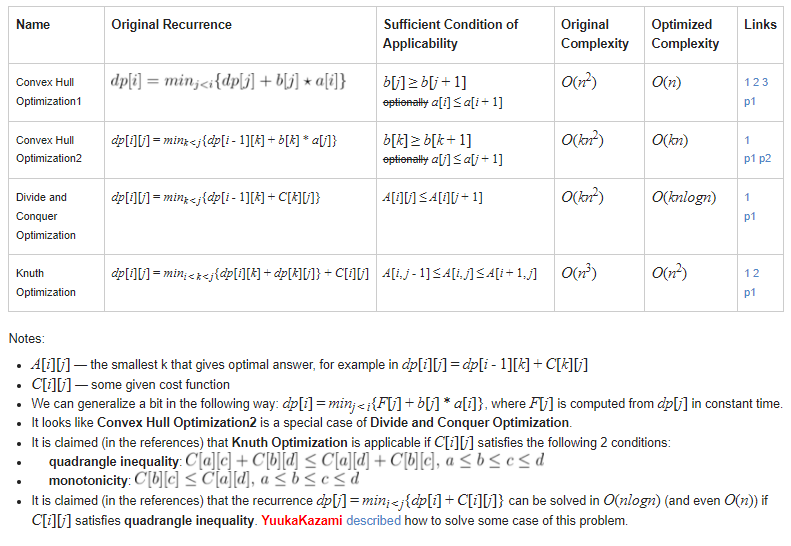
\includegraphics{solutions/DP/dpo.png}
    \subsection{D\&C}
    
    \lstinputlisting{./solutions/DP/divideandconquer.cpp}
    \subsection{Knuth Optimization}
    \lstinputlisting{./solutions/DP/knuth_optimization.cpp}
    \subsection{Convex Hull Trick}
        \subsubsection{Convex Hull Trick 1}
        This solutions only works when the coefficients are all increasing / decreasing, and the queries decreasing / increasing. Improve $O(n^2)$ to $O(n)$. (Original Problem: Codeforces - Round 189 (Div. 1) C)
        \lstinputlisting{./solutions/DP/ConvexHull1.cpp}
        
        \subsubsection{Convex Hull Trick 2}
        This solutions works under the same conditions for Convex Hull Trick 1, but it's used to solve problems in a 2D dynamic programming, like problem NKLEAVES from spoj. In resume we need to group $N$ leaves in $K$ groups, for each coordinate between 1 and $N$ there is a leaf with weight $w_i$, and the leaves can only be moved to the left, and the cost is $w_i * d$ where $d$ is the distance that leaf $i$ was moved. The problem asks for minimum cost to group the $N$ leaves in $K$ groups. Lets reverse the leaves weights, now the leafs can only be moved to the right.
        
        So, the recurrence is:
        
        \bigskip
        
        $dp_{i, j} = \min_{k \leq i} ( (\sum_{p=k}^{i} (i - p) * w_p) + dp_{k - 1, j - 1})$, clearly $O(n^2k)$
        
        \bigskip
        
        So we will keep our lines in such way, that we can solve this problem, see the code below. 
        
        This solutions only works when the coefficients are all increasing / decreasing, and the queries decreasing / increasing. Improve $O(n^2k)$ to $O(nk)$. (Original Problem: SPOJ - NKLEAVES)
        
        \lstinputlisting{./solutions/DP/ConvexHullTrick2.cpp}
        
        \subsubsection{Convex Hull Trick 3 (Online Queries)}
        This solutions works without any assumption about the coeficients, in this case we will query is answered in $O(logn)$.
        
        Improve $O(n^2)$ to $O(nlogn)$. (Original Problem: Codeforces - Round 463 div1+div2 F. Escape Through Leaf)
        
        \lstinputlisting{./solutions/DP/ConvexHullTrick3.cpp}
        
    \section{Steiner Tree DP}

    MST for a subset
    
    \lstinputlisting{./solutions/DP/SteinerTree.cpp}
    
 \chapter{String}
    
    % \section{AHO - TBD}
    % \section{ZFUNCTION TBD}
    \section{String Hash}
    Compare two strings in $O(1)$ time, with $O(N)$ time preprocessing.
    \subsection{Simple Hash}
    \lstinputlisting{./solutions/String/StringHash.cpp}
    \subsection{Hash 2D$_{\text{ayllon}}$}
    Cuidado, a hash é dupla, pode dar TLE!
    As string são indexados de 0!
    Apenas dentro da hash que setamos para ser idexado de 1 (igual string hash normal).

    Problema resolvido: Dado duas matrizes de char, achar as posições das ocorrências da primeira matriz na segunda.
    \lstinputlisting{./solutions/String/StringHash2Dayllon.cpp}

    \subsection{Hash 2D - Gustavo}
    esse código ta horroroso
    \lstinputlisting{./solutions/String/StringHash2D.cpp}
    \subsection{Hash 2D}
    Tudo é indexado de 1
    \lstinputlisting{./solutions/String/StringHash2D-Impl2.cpp}

    \subsection{Hash with Updates}

    For this problem, the idea is that you can compare the hashes of the string and it's reversed one to discover if it is a palindrome. To do the updates, just use some data structure that allows point update and range queries. The one below uses a BIT.
    \lstinputlisting{./solutions/String/Palindrome_Queries.cpp}
    
    \section{Suffix Array}
    The key idea is to make a substring problem, into a prefix problem.
    Remember to add a '\#' at the end of the string.
    Another important fact is that $lcp(i,j) = min_{k=i}^{j-1} lcp[k]$.
    \lstinputlisting{./solutions/String/SuffixArray.cpp}
    \section{Suffix Automaton}
    The key idea is to make a substring problem, into a DAG problem.
    
    link points to the greatest suffix
    
    Most of harder problems,  you can just sort the states by len, and walk from greater to smaller
    making some updates in a dp like style.

    \lstinputlisting{./solutions/String/SuffixAutomaton.cpp}
    
    Example 1:

    You are given a string of length $n$. If all of its substrings (not necessarily distinct) are ordered lexicographically, what is the $k$-th smallest of them?

    DP to count Paths(remember its a DAG) then just do a walk. Easier version doesnt need to count repetitions, so just a path.

    \lstinputlisting{./solutions/String/SubstringOrderII.cpp}
    
    Example 2:
    
    You are given a string of length n. For every integer between 1…n you need to print the number of distinct substrings of that length.

    
    \lstinputlisting{./solutions/String/SubstringDistribution.cpp}
    
    Example 3:

    A repeating substring is a substring that occurs in two (or more) locations in the string. Your task is to find the longest repeating substring in a given string.
    
    \lstinputlisting{./solutions/String/RepeatingSubstring.cpp}
    
    \section{Suffix Tree} 
    The idea is that you transform a string problem into a tree problem, so you can use tree techniques to solve it, like LCA, Euler Tour, DP on Trees, and many others.
    
    (Original Problem SPOJ - TOP 10).
    \lstinputlisting{./solutions/String/SuffixTree.cpp}
    \section{Palindromic Tree} 
    \lstinputlisting{./solutions/String/PalinTree.cpp}
    \section{Minimal Rotation}
    Find the minimal cyclic shift of an string in O(N).
    
    \lstinputlisting{./solutions/String/SmallestCyclicShift.cpp}
    \section{Aho Corasick} 
    This aho has the shape of the Suffix Automaton, mos of things that can be done in there, can be done here as well(sort by len and do something using links).

    \lstinputlisting{./solutions/String/aho.cpp}
    
    
    
 \chapter{Graph}
    \section{Flow}
    \subsection{Teoremas de Fluxo}
    \begin{itemize}
        \item \textbf{Corte mínimo:}
        \begin{itemize}
            \item Valor do fluxo máximo é igual ao valor do corte mínimo.
        \end{itemize}
        \item \textbf{Emparelhamento:}
        \begin{itemize}
            \item O emparelhamento máximo em um grafo bipartido é igual ao fluxo máximo.
        \end{itemize}
        \item \textbf{Teorema Berge (1957):}
        \begin{itemize}
            \item Seja $G=(V, E)$ um grafo. Um emparelhamento $M \subseteq E$ é máximo se não há caminhos aumentantes.
        \end{itemize}
        \item \textbf{Teorema Hall (1935):}
        \begin{itemize}
            \item Seja $G$ um grafo bipartido com bipartição $(X, Y)$. Então $G$ admite um emparelhamento que satura todos os vértices de $X$ se e somente se $|N(S)| \ge |S|$ para todo $S \subseteq X$.
            \item $|N(x)|$, para algum $x \in V$, é o conjunto vizinhança do vértice $x$, isto é, $|N(x)| = \{y,$ para todo $y$ tal que existe $(x, y)\in E\}$.
            \item $N(S)=\underset{s\in S}{\cup} N(s)$.
        \end{itemize}
        \item \textbf{Teorema Tutte}
        \begin{itemize}
            \item $G$ tem um emparelhamento perfeito se e somente se $i(G-S) \le |S|$, para todo $S \subseteq V(G)$.
            \item Uma componente de um grafo é ímpar/par se possui um número ímpar/par de vértices. Denotaremos por $i(G)$ o número de componentes ímpares de um grafo $G$.
        \end{itemize}
        \item \textbf{Teorema Kőnig-Egerváry (1931):}
        \begin{itemize}
            \item Seja $G=(V, E)$ um grafo bipartido. Então cobertura($G$) $=$ emparelhamento($G$).
            \item Let 
$\displaystyle (S,T)$ be a minimum cut. Let 
$\displaystyle A=A_{S}\cup A_{T}$ and 
$\displaystyle B=B_{S}\cup B_{T}$, such that 
$\displaystyle A_{S},B_{S}\subset S$ and 
$\displaystyle A_{T},B_{T}\subset T$. Then the minimum cut is composed only of edges going from
$\displaystyle s$ to 
$\displaystyle A_{T}$ or from 
$\displaystyle B_{S}$ to 
$\displaystyle t$, as any edge from 
$\displaystyle A_{S}$ to 
$\displaystyle B_{T}$ would make the size of the cut infinite.

Therefore, the size of the minimum cut is equal to 
$\displaystyle |A_{T}|+|B_{S}|$. On the other hand, 
$\displaystyle A_{T}\cup B_{S}$ is a vertex cover, as any edge that is not incident to vertices from 
$\displaystyle A_{T}$ and
$\displaystyle B_{S}$ must be incident to a pair of vertices from 
$\displaystyle A_{S}$ and 
$\displaystyle B_{T}$, which would contradict the fact that there are no edges between 
$\displaystyle A_{S}$ and 
$\displaystyle B_{T}$.
Thus, 
$\displaystyle A_{T}\cup B_{S}$ is a minimum vertex cover of 
$\displaystyle G$.
\item basically just check if the cut was on a edge related to $S$ or to $T$.
        \end{itemize}
        \item \textbf{Teorema Independência:}
        \begin{itemize}
            \item Seja $G=(V, E)$ um grafo. Então independência($G$) $=$ $n - $ cobertura($G$).
        \end{itemize}
        \item \textbf{Teorema Menge (1927):}
        \begin{itemize}
            \item Seja $D=(V, E)$ um grafo direcionado e $s,t \in V$ dois vértices distintos. Então o número máximo de $st$-caminhos disjuntos nas arestas é igual ao número mínimo de arestas cuja remoção impossibilita a existência de $st$-caminhos.
            \item Seja $D=(V, E)$ um grafo direcionado e $s,t \in V$ dois vértices distintos. Então o número máximo de $st$-caminhos disjuntos nos vértices é igual ao número mínimo de vértices cuja remoção impossibilita a existência de $st$-caminhos.
            \item Seja $D=(V, E)$ um grafo direcionado, onde toda aresta tem capacidade $1$, e $s,t \in V$ dois vértices distintos. Seja $f^*$ o fluxo máximo e seja $K^*$ um corte mínimo separador. Então:
            \begin{itemize}
                \item val($f^*$) $=$ número máximo de caminho disjuntos nas arestas.
                \item cal($K^*$) $=$ número mínimo de arestas em $D$ cuja remoção impossibilita a existência de $st$-caminhos.
            \end{itemize}
        \end{itemize}
    \end{itemize}

    \begin{itemize}
        \item \textbf{Observações:}
        \begin{itemize}
            \item Dá pra usar um monte de gambiarra junto com Fluxo, tipo Dijkstra, Busca Binária, perceber que a vizinhança é igual e juntar elas de algum jeito, entre outras.
        \end{itemize}
    \end{itemize}
    
    \subsection{Dinic}
        \lstinputlisting{./solutions/Graph/dinic.cpp}
    \subsection{MinCostMaxFlow}
            The problem is given a Graph with a source and sink vertices, each edge has a capacity $c_i$ and cost $l_i$ per unit of flow, compute the minimum cost to transport a max flow in this network.

            \lstinputlisting{./solutions/Graph/mcmf.cpp}

    \section{Matching}
         \subsection{HopCroft Karp}
            Compĺexity for sparse graphs $O(E log(V))$
            Compĺexity for dense graphs $O(E sqrt(V))$
            \lstinputlisting{./solutions/Graph/non_weighted_bipartite_matching.cpp}
        \subsection{Bipartide Weighted Hungarian Method}
        Compĺexity $O(V^3)$
        \lstinputlisting{./solutions/Graph/hungarian.cpp}
        \subsection{General Graph (Edmonds Blossom)}
        Complexity $O(VE^2)$
        \lstinputlisting{./solutions/Graph/MatchGeneral.cpp}
    \section{Bellman Ford}
        Algorithm used to calculate minimal distance with negative edges. In this Problem you need to find the minimal path(actually it is maximal) from 1 to n and if it is infinite you need to print "-1".
        There is a important point, that is, a infinite path starting at 1, can actually stop in a sub-graph and don't go to N. A smart way  to deal with it is using bellman ford again.

        \lstinputlisting{./solutions/Graph/HighScore.cpp}
    \section{2-SAT}
    In a 2-SAT, all states should be a in conjunctive normal form, so we can see as a and of or's.

    \begin{itemize}
        \item $ a \lor b = a \lor b$
        \item $ a \land b = (a \lor a) \land (b \lor b)$
        \item $ \neg a = \neg a \lor \neg a$
        \item $ a = a \lor a$
        \item $ a \oplus b = (a \lor b) \land (\neg a \lor \neg b)$
        \item $ \neg (a \oplus b) = (\neg a \lor b) \land (\neg b \lor a)$
        \item $ a \Rightarrow b = \neg a \lor b$
    \end{itemize}
    
    \lstinputlisting{./solutions/Graph/2SAT.cpp}

    \section{Componentes Fortemente Conexas}

    Uma componente é dita fortemente conexa se podemos sair de u para v e de v para u. Um grafo das componentes fortemente conexas é a condensação de cada componente em um vértice, e isso sempre vira uma DAG. Dá pra usar algoritmos clássicos de resolver problemas em uma DAG dps de condensar o grafo.

    Aqui tem um algoritmo que faz isso. De autoria do grande Wevton Santana, o inconfiável.
    
    \lstinputlisting{./solutions/Graph/SCC.cpp}

    \section{Stable Marriage}

    Given $n$ men and $n$ women, where each person has ranked all members of the opposite sex in order of preference, marry the men and women together such that there are no two people of opposite sex who would both rather have each other than their current partners. When there are no such pairs of people, the set of marriages is deemed stable.
    
    Someone way before my father was born proved that it is always possible to match everyone if there are equal numbers of men and women, and that all marriages in the end are stable. The algorithm presented below works in $\mathcal{O}(n^2)$.

    \lstinputlisting{./solutions/Miscellaneous/StableMarriage.cpp}
    
    \section{Planar Graphs}
    Some theorems related to planar graphs. Most of them constraints conditions between the quantity of vertices $v$, the quantity of edges $e$ and the quantity of faces $f$.
    \begin{itemize}
        \item $v - e + f = 2$
        \item $e \leq 3*v - 6$
        \item $D = \frac{f-1}{2*v-5}$
        \item every planar graph is 4-colourable.
        \item a really dense(maximal) planar graph has $3*v-6$ edges and $2*v-4$ faces.
    \end{itemize}
    \section{Dominator Tree}
    \begin{itemize}
        \item Dominator : Dominators are defined in a directed graph with respect to a source vertex $S$. Formally, A node $u$ is said to dominate a node $w$ when related to a source vertex $S$ if all the paths from $S$ to $w$ in the graph must pass through node $u$.
        \item Immediate Dominator : A node $u$ is said to be an immediate dominator of a node $w$ (denoted as $idom(w)$) if $u$ dominates $w$ and every other dominator of $w$ dominates $u$ (every vertex have only one immediate dominator).
        \item Dominator Tree :  The edges $\big\{(idom(w),w) \mid w \epsilon V - \big\{S\big\} \big\}$ forms a directed tree with $S$ being the root of the tree.
    \end{itemize}
    
    Note that only the vertices that are reachable from source vertex in the directed graph are considered here. It is assumed that every vertex in the graph is reachable from the source.

    The problem using the structure is Critical Cities, CSES.
    It is related to find all dominators from n, when S = 1.
    \lstinputlisting{./solutions/Graph/dominator.cpp}

    \section{Chinese Postman Problem}
    The problem is, given a undirected weighted graph, find a tour that visits each edge at least one time, and the sum of weights from visited edges is minimum as possible.
    $O(2^n.n)$ where $n$ is the number of vertices. (Original Problem - UVa 10296 - Jogging Trails)
    
    \lstinputlisting{./solutions/Graph/JoggingTrails.cpp}
    
    \section{Some Bridge related topics}
    \subsection{Finding Bridges}
    just check if the lowest back edge of the bottom most vertex off an edge in a dfs tree entered in a time later than the time the top most vertex entered the dfs.
    \lstinputlisting{./solutions/Graph/bridges.cpp}
    \subsection{Articulation Points}
    Points which when removed create multiple graphs.
    The main idea is the same of finding bridges, utilize the low to check somethings in the dfs tree.
    \lstinputlisting{./solutions/Graph/articulation.cpp}

    \subsection{Block Cut Tree}
    \begin{center}
        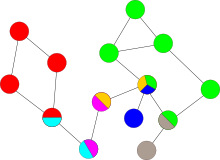
\includegraphics[]{imgs/bicomp.png}
    \end{center}
    Construct a tree of bi-connected components of the graph.
    Some of the approaches related to this structure needs you to do some updates in the parent of the node.

    The application is a problem with a lot of queries
    each query will give 3 vertices a b and c and ask if there is a path that goes from a to b, without passing in c.
    The answer is no if a ==b, a == c or c is an articulation point and is in the path of the block cut tree going from a to b.
    \lstinputlisting{./solutions/Graph/block_cut_tree.cpp}

    \subsection{Two Edge Connected Components}
    Decompose the graph in Components connected by at least two edges.
    Can be used to create a tree as well. a "block cut" decomposition, but with edges instead of vertices.

    \lstinputlisting{./solutions/Graph/2cc.cpp}

    

    
 \chapter{Trees}
    \section{Diameter}
    Finding the diameter of the tree. Just do two DFS's, where in the first one u find the longest guy u can reach, and then find the other guy starting from the one you found before.
    \lstinputlisting{./solutions/Tree/diameter.cpp}
    \section{LCA}
    A way to find the lowest common ancestor of two vertex $(a,b)$ in a tree. Needs a Sparse Table.
    \lstinputlisting{./solutions/Tree/lca.cpp}
    Version that Sabino likes
    \lstinputlisting{./solutions/Tree/lca2.cpp}

    
    \section{Euler tour tree}

    No code here, use lca code. remember u can calc paths using the ett. There are two types.
    
    Incrementing $out$, and not incrementing $out$. We can use the first one as a kind of bit with $f(x)$ in $in[x]$ and $f(x)^{-1}$ in $out[x]$
    
    \section{Small to Large}

    Not much to say, the code is always different, so lets just keep the USACO text:

    Naive Solution

    Suppose that we want merge two sets $a$ and $b$ of sizes $n$ and $m$,
    respectively. One possibility is the following:
    
    \lstinline{for (int x : b) a.insert(x);}
    
    which runs in $\mathcal{O}(m\log (n+m))$ time, yielding a runtime of
    $\mathcal{O}(N^2\log N)$ in the worst case. If we instead maintain $a$ and $b$
    as sorted vectors, we can merge them in $\mathcal{O}(n+m)$ time, but
    $\mathcal{O}(N^2)$ is also too slow.
    
    Better Solution
    
    With just one additional line of code, we can significantly speed this up.
    
    \lstinline{if (a.size() < b.size()) swap(a, b);for (int x : b) a.insert(x);}
    
    Note that swap exchanges two
    sets in $\mathcal{O}(1)$ time. Thus, merging a smaller set of size $m$ into the
    larger one of size $n$ takes $\mathcal{O}(m\log n)$ time.
    
    Claim: The solution runs in $\mathcal{O}(N\log^2N)$ time.
    
    Proof: When merging two sets, you move from the smaller set to the larger
    set. If the size of the smaller set is $X$, then the size of the resulting set
    is at least $2X$. Thus, an element that has been moved $Y$ times will be in a
    set of size at least $2^Y$, and since the maximum size of a set is $N$ (the
    root), each element will be moved at most $\mathcal{O}(\log N$) times.

    Generalizing

    We can also merge other standard library data structures such as std::map or
    std:unordered\_map in the same way. However,
    std::swap does not always
    run in $\mathcal{O}(1)$ time. For example, swapping
    std::arrays takes time
    linear in the sum of the sizes of the arrays, and the same goes for
    GCC policy-based data structures such
    as \_\_gnu\_pbds::tree or \_\_gnu\_pbds::gp\_hash\_table.
    
    To swap two policy-based data structures a and b in $\mathcal{O}(1)$ time,
    use a.swap(b) instead. Note that for standard library data structures,
    swap(a,b) is equivalent to a.swap(b).
    
    \section{HLD}
    You are given a tree consisting of n nodes. The nodes are numbered 1,2,…,n. Each node has a value.

    Your task is to process following types of queries:
    \begin{itemize}
        \item Change the value of node s to x
        \item Find the maximum value on the path between nodes a and b.
    \end{itemize}

    \lstinputlisting{./solutions/Tree/PathQueriesII.cpp}
    \subsection{Can you answer these queries VII}
        Given are a tree with $n$ vertices, each vertice has a weight $x_i$, and two type of operations. Operation 1 asks for the maximum contiguous sum between two vertices $a$ and $b$. Operation 2 update the values of vertices between $a$ and $b$ to $c$. We have to process $Q$ operations.
        
        The problem can be solved with HLD in $O(Q(log(n))^2)$. Original Problem (SPOJ - GSS7).
        
        \lstinputlisting{./solutions/Tree/HLD.cpp}
        
        \subsection{Can you answer these queries VI}
        Given a tree with $n$ vertices, each vertice has a color (0 or 1), and two type of operations. Operation 0 asks for how many vertices are connected to a vertice $u$, when one vertice $v$ is connected to $u$ only if the path between $u$ and $v$ just contain vertices with same color of $u$ inclusive. Operation 1 is to change the color of vertice $u$ (0 to 1 and 1 to 0).
        
        The problem can be solved wih HLD in $O(Q(log(n))^2)$. Original Problem (SPOJ - Can You Answer These Queries VI).
        
        
        \lstinputlisting{./solutions/Tree/CanYouAnswerTheseQueriesVI.cpp}

         \subsection{HLD with subtree queries}
        Slower version with subtree queries, uses lazy segtree and  template
        
        
        \lstinputlisting{./solutions/Tree/HLD_subtree.cpp}
    \section{Centroid Decomposition}


    Always about path problems.
    
    There are two types of centroid solving. Do some computation during centroid and use it.
     Or keep some data for each node and make updates in $O(log(N))$. 

    \lstinputlisting{./solutions/Tree/centroid.cpp}

    Version that Sabino likes

    \lstinputlisting{./solutions/Tree/centroid2.cpp}

    Example 1:
    Given a tree of $n$ nodes, your task is to count the number of distinct paths that consist of exactly $k$ edges.

    \lstinputlisting{./solutions/Tree/FixedLengthPathsI.cpp}
    
    Example 2: 
    Xenia has a tree consisting of $n$ nodes. We will consider the tree nodes indexed from $1$ to $n$. We will also consider the first node to be initially painted red, and the other nodes — to be painted blue.
    
    execute queries of two types:
    \begin{itemize}
        \item paint a specified blue node in red;
        \item calculate which red node is the closest to the given one and print the shortest distance to the closest red node.
    \end{itemize}

    \lstinputlisting{./solutions/Tree/xenia&tree.cpp}
    
    
    \section{Tree Isomorphism}

    In this code, we generate an id for each tree.
    It is also possible to do with subtrees.

    \lstinputlisting{./solutions/Tree/treehash.cpp}

    \section{Virtual Tree}
    A different way to approach trees problems. Main idea here is to create a tree with the "relevant nodes". Normally related to colors and problems which we solve looking for each color at a time.

    
    \lstinputlisting{./solutions/Tree/virtual_tree.cpp}
    
    
    \section{Link Cut Tree}
    A link cut tree is a data structure that uses splay trees to represent a forest of rooted trees and can perform the following operations with an amortized upper bound time complexity of $\mathcal{O}(\log N)$:
    \begin{itemize}
        \item Linking a tree with a node by making the root of the tree a child of any node of another tree
        \item Deleting the edge between a node and its parent, detaching the node's subtree to make a new tree
        \item Find the root of the tree that a node belongs to
    \end{itemize}

    These operations all use the $\texttt{access}(v)$ subroutine,
which creates a preferred path from the root of the represented tree to vertex $v$, making a corresponding auxiliary splay tree with $v$ as the root.

    \lstinputlisting{./solutions/Tree/linkcut.cpp}
    
    
    
\chapter{Geometry}
    \section{Simple Geometry}
    This section will have alot of functions used in geometry problems. They are related to points, lines, circles and polygons.
    \subsection{Points and Lines}
    This is the base of all codes in geometry. u can change the type from ldb to ll and also change the EPS. The rest is pretty much fixed.
    \lstinputlisting{./solutions/Geometry/base.cpp}
    \subsection{Circles}
    This section will have alot of algorithms related to circles and their description
    A circle will have the following format:
    \begin{lstlisting}
    typedef pair<pt, T> circle;
    \end{lstlisting}
    
    
    To see if a point is in/on/out a circle we can do:
    \begin{lstlisting}
// -1 if inside, 0 if in border, 1 if outside
int in(const circle& x, const pt& y) { 
    return sgn(abs(y-x.ft)-x.sd); 
 }
    \end{lstlisting}
    Arc length of two points:

    \begin{center}
    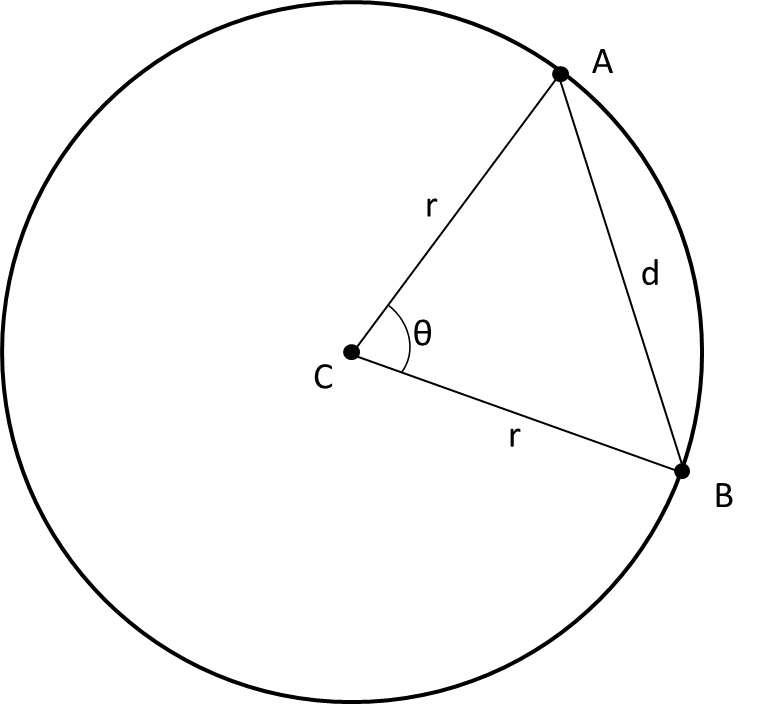
\includegraphics[scale = 0.5]{imgs/arclength.png}
    \end{center}
    
    \begin{lstlisting}
T arcLength(const circle& x, pt a, pt b) {
    // precondition: a and b on x
    pt d = (a-x.ft)/(b-x.ft); return x.sd*acos(d.ft); 
}
    \end{lstlisting}
    
    Intersections related to circles:
    \begin{lstlisting}
vpt isect(const circle& x, const circle& y) { // precondition: x!=y
    T d = abs(x.ft-y.ft), a = x.sd, b = y.sd; 
    if (sgn(d) == 0) { assert(a != b); return {}; }
    T C = (a*a+d*d-b*b)/(2*a*d); 
    if (abs(C) > 1+EPS) return {};
    T S = sqrt(max(1-C*C,(T)0)); 
    pt tmp = (y.ft-x.ft)/d*x.sd;
    return {x.ft+tmp*pt(C,S),x.ft+tmp*pt(C,-S)};
}

vpt isect(const circle& x, const line& y) {
    pt c = foot(x.ft,y); 
    T sq_dist = sq(x.sd)-abs2(x.ft-c);
    if (sgn(sq_dist) < 0) return {};
    pt offset = unit(y.sd-y.ft)*sqrt(max(sq_dist,T(0)));
    return {c+offset,c-offset};
}

T isect_area(circle x, circle y) { // not thoroughly tested
    T d = abs(x.ft-y.ft), a = x.sd, b = y.sd; 
    if (a < b) swap(a,b);
    if (d >= a+b) return 0;
    if (d <= a-b) return PI*b*b;
    T ca = (a*a+d*d-b*b)/(2*a*d), cb = (b*b+d*d-a*a)/(2*b*d);
    T s = (a+b+d)/2, h = 2*sqrt(s*(s-a)*(s-b)*(s-d))/d;
    return a*a*acos(ca)+b*b*acos(cb)-d*h;
}
    \end{lstlisting}

    A tangent to a circle is a line in the plane of a circle which intersects the circle in exactly one point. This point is called the point of tangency.

    A tangent of two circles is a common internal tangent if the intersection of the tangent and the line segment joining the centers is not empty.

    \begin{center}
    \begin{minipage}{.5\textwidth}
    \centering
    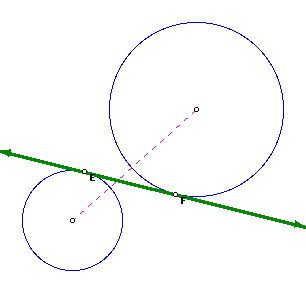
\includegraphics[scale = 0.5]{imgs/internal1.png}
    \end{minipage}%
    \begin{minipage}{0.5\textwidth}
    \centering
    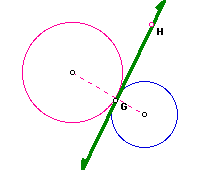
\includegraphics[scale = 0.5]{imgs/internal2.png}
    \end{minipage}
    \end{center}
    
    
    A tangent of two circles is a common external tangent if the intersection of the tangent and the line segment joining the centers is empty.

    
    \begin{center}
    \begin{minipage}{.5\textwidth}
    \centering
    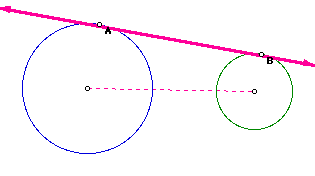
\includegraphics[scale = 0.5]{imgs/external1.png}
    \end{minipage}%
    \begin{minipage}{0.5\textwidth}
    \centering
    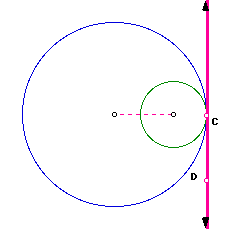
\includegraphics[scale = 0.5]{imgs/external2.png}
    \end{minipage}
    \end{center}
    
    \begin{lstlisting}
pt tangent(pt x, circle y, int t = 0) {
	y.sd = abs(y.sd); // abs needed because internal calls y.s < 0
	if (y.sd == 0) return y.ft;
	T d = abs(x-y.ft);
	pt a = pow(y.sd/d,2)*(x-y.ft)+y.ft;
	pt b = sqrt(d*d-y.sd*y.sd)/d*y.sd*unit(x-y.ft)*dir(PI/2); 
	return t == 0 ? a+b : a-b;
}
vector<pair<pt,pt>> external(circle x, circle y) { 
	vector<pair<pt,pt>> v; 
	if (x.sd == y.sd) {
		pt tmp = unit(x.ft-y.ft)*x.sd*dir(PI/2);
		v.eb(x.ft+tmp,y.ft+tmp);
		v.eb(x.ft-tmp,y.ft-tmp);
	} else {
		pt p = (y.sd*x.ft-x.sd*y.ft)/(y.sd-x.sd);
		rep(i, 0, 2) v.eb(tangent(p,x,i),tangent(p,y,i));
	}
	return v;
}
vector<pair<pt,pt>> internal(circle x, circle y) { 
	return external({x.ft,-x.sd},y); }
    \end{lstlisting}

    The CircumCenter of a triangle is the minimum enclosing circle of a triangle.
    We can also calculated the minimum enclosing circle of a polygon.

    \begin{center}
    \begin{minipage}{.3\textwidth}
    \centering
    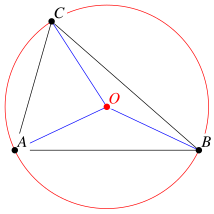
\includegraphics{imgs/circumcenter.png}
    \end{minipage}%
    \begin{minipage}{0.7\textwidth}
    \centering
    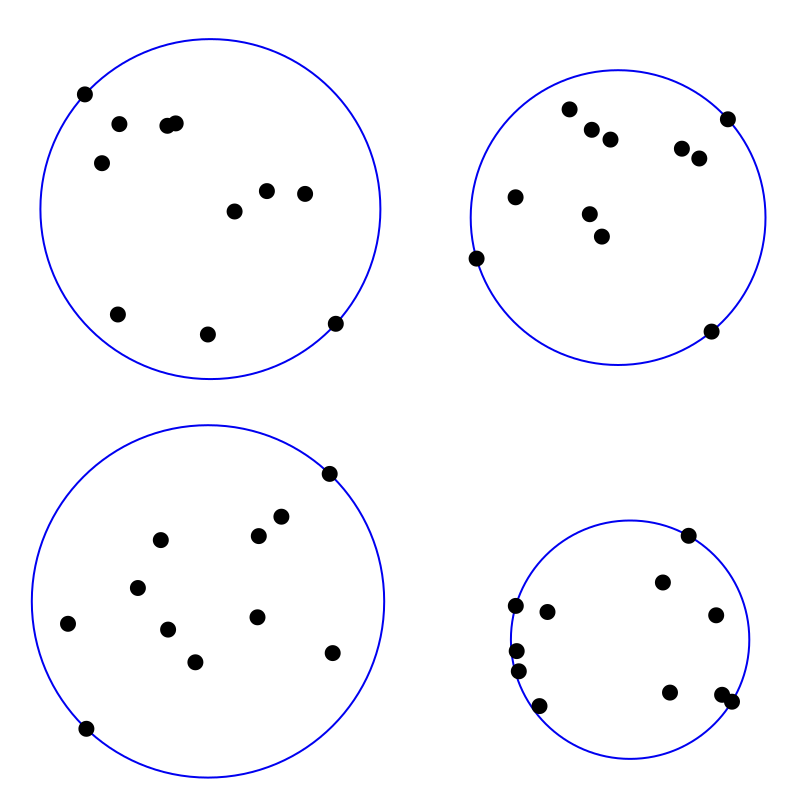
\includegraphics[scale = 0.5]{imgs/mec.png}
    \end{minipage}
    \end{center}
    

    
    \begin{lstlisting}
// return the minimum enclosing circle of a triangle
circle ccCenter(pt a, pt b, pt c) { 
	b -= a; c -= a;
	pt res = b*c*(conj(c)-conj(b))/(b*conj(c)-conj(b)*c);
	return {a+res,abs(res)};
}

// return the minimum enclosing circle of a set of points O(N)
circle mec(vpt ps) {
	shuffle(all(ps), rng);
	pt o = ps[0]; 
    T r = 0, EPS = 1+1e-8;
	rep(i, 0, (int)ps.size()) 
        if (abs(o-ps[i]) > r*EPS) {
            o = ps[i], r = 0; // point is on MEC
            rep(j, 0, i) 
                if (abs(o-ps[j]) > r*EPS) {
                    o = (ps[i]+ps[j])/2, r = abs(o-ps[i]);
                    rep(k, 0, j) if (abs(o-ps[k]) > r*EPS) 
                        tie(o,r) = ccCenter(ps[i],ps[j],ps[k]);
                }
        }
	return {o,r};
}
    \end{lstlisting}
    \section{Convex Hull}
        \subsection{Rotation Calipers}
        Diameter from a convex Polygon.
        
        Solution $O(n)$. Original Problem (NCPC 2013 - D).
        
        \ \\
        
        \begin{tabular}{|p{31cm}|}
          \begin{verbatim}
            Implementacao do Convex Hull do CP-ALGORITHMS
            Para usar crie um vetor com os pontos,
            		vector<pt> pts;
            e execute
            		convex_hull(|pts|);
            Apos isso, o vector pts sera alterado e ele so tera os pontos do Convex Hull 
            na ordem horaria, comecando do elemento de menor x, como segunda condicao menor y.
            
            Como funciona o algoritmo
            - Acha os dois extremos de x.
            - Monta dois subgrupos, os "up" e os "down", em relacao
            Convex Hull na parte superior e inferior.
            - Itera pelos pontos e usa o produto vetorial para ver se
            ele forma um sentido horario, se formar adiciona.
            - Remove todos os anteriores ao ultimo ponto adicionado que agora, com o ponto
            atual, formando um sentido anti-horario
            \end{verbatim}
        \end{tabular}
        \\
        
        \lstinputlisting{./solutions/Geometry/MaxDistanceBetweenPoints.cpp}
        
    \section{Line Sweep}
        \subsection{Points Inside Triangles}
        Given $n$ triangles with vertices {($x_i$, $y_i$), ($x_i + d$, $y_i$), ($x_i$, $y_i + d$)}, and $q$ points, compute for each triangle, the number of points that lie inside or in boundary of him. $O(nlogn)$. (Original Problem: CODECHEF - TRIANGULAR QUERIES)
        \lstinputlisting{./solutions/Geometry/PointsInsideTriangles.cpp}
        \newpage
        \subsection{Ranking Problem}
        Given $n$ students that attended to $3$ contests, and all of them have different ranks, between $1$ and $n$ inclusive, for each contest. We say that one student $a$ is better that student $b$, if all ranks of student $a$ in each contest is lesser that student $b$. A student is said to be excellent if no other student is better than him. How many excelent students there exists ?
        
        This solutions runs in $O(nlogn)$. (Original Problem: SPOJ: NICEDAY)
        
        \lstinputlisting{./solutions/Geometry/RankingProblem.cpp}
        \newpage
        \subsection{Balls Falls and Segments}
        Given $n$ segments (non horizontal and with no common points), and $m$ balls in a 2D plane, say for each ball the x point which he falls. (This solution was upload, the source code is just for only one ball, but the overall complexity is still $O(nlogn)$ if the number of balls is $O(n)$).
        
        This solutions runs in $O(nlogn)$. Original Problem (NCPC 2013 - H).
        
        \lstinputlisting{./solutions/Geometry/WaterFalls.cpp}
        \newpage
        \subsection{Checking Points Inside Convex Polygon}
            % \subsubsection{Offline}
            % Given $n$ points in 2D plane, and a Convex Polygon, check for each of these $n$ points, if them are strict inside or not of polygon.
            
            % This solutions runs in $O(nlogn)$ but i used Fracion Class to Take Care with double error precisions, so the overall solution in this case is $O(nlogn^2)$.
            
            % \lstinputlisting{./solutions/Geometry/PointsInsideConvexPolygon.cpp}
            % \newpage
            \subsubsection{Online}
            Given one point and a Convex Polygon, with vertices in counter clockwise order, check if this point is inside or in boundary of him.
            
            This solutions runs in $O(logn)$.
            
            \lstinputlisting{./solutions/Geometry/PointsInsideConvexPolygonOn.cpp}
        % \newpage
        % \subsection{Area of Rectangles Union}
        % Given a set of N axis aligned rectangles, you need to find the area of their union. Each rectangle is represented by two points, one lower-left point and one upper-right point. The coordinates are all integers.
        
        % This solutions runs in $O(nlogn)$. Original Problem (HackerEarth - Line Sweep Tutorial, Sample Exercicise)
        
        % \lstinputlisting{./solutions/Geometry/RectangleUnion.cpp}
        % \newpage
        \subsection{Radial Sweep}
        You are given $N$ red points and $M$ blue points on a 2D plane.

        You are required to delete the minimum number of points(the deleted points can be of both colors) so that it's possible to draw a line such that all remaining red points are on one side of the line while all remaining blue points are on the other side of the line.
        
        This solutions runs in $O(n^2logn)$. Original Problem (Codechef, REDBLUE - DEC17)
        
        \lstinputlisting{./solutions/Geometry/RadialSweep.cpp}
        \subsection{Radial Sweep sem Double}
        You are in a point inside a square NxN. There are some rocks(polygons) inside the square, u need to discover how many points form the perimeter of the square, are visible, form your oirigin
    
        In this problem, there are three types of events: when our ray hits a fence point, enters a rock, or exits a rock.

    The second and third types of events can be found for each rock by sorting the rays to its vertices by bearing and then taking the two endpoints of the sorted list. These two rays are the two tangents to the rock.
    
    We can then perform a radial sweep to find the fence posts that Farmer Don can see - these fence posts are simply the ones where the number of type-2 and type-3 events we've processed so far are equal.
        
        \lstinputlisting{./solutions/Geometry/SeeingTheBoundary.cpp}
    % \newpage
    \section{Minimum Perimeter Triangle}
    Given $n$ points in a 2D plane, return the minimum perimeter that can be formed taking three points, collinear points are allowed. $O(nlogn)$. (Original Problem - Google Code Jam WF 2009 - B)
    \lstinputlisting{./solutions/Geometry/MinPerimeterTriangle.cpp}
    % \section{Line Sweep}
    
    
    
 \chapter{Miscellaneous}
    \section{Game Theory}
        Pontos importantes:
        \begin{itemize}
            \item \textit{Teoria do Espelhamento}: Se o seu oponente pode espelhar todas as suas ações, este é um estado de derrota.
            \item Dois nim games são combinados usando o XOR.
            \item Podem existir ciclos modulares, vale brutar.
            \item Em algum momento pode se tornar sempre win, ou sempre loss.
            \item Se a gente transformar o problema num nim, podemos usar o teorema de grundy, que basicamente é achar os casos derrota + fazer o mex.
        \end{itemize}
        
        Example 1:

        There is a heap of $n$ coins and two players who move alternately. On each move, a player chooses a heap and divides into two nonempty heaps that have a different number of coins. The player who makes the last move wins the game.

        Here for big N the answer is always first.

        
    \lstinputlisting{./solutions/Miscellaneous/GrundyGame.cpp}

        Example 2:

        There is a staircase consisting of $n$ stairs, numbered $1,2,\ldots,n$. Initially, each stair has some number of balls.

        There are two players who move alternately. On each move, a player chooses a stair $k$ where $k\neq1$ and it has at least one ball. Then, the player moves any number of balls from stair $k$ to stair $k-1$. The player who moves last wins the game.

        Here, every odd position is losing, u can see them as "dark holes", using the "Teoria do Espelhamento", so it's just N/2 Nim games.

        
    \lstinputlisting{./solutions/Miscellaneous/StairGame.cpp}

    \subsection{Nim Multiplication}
        A 2D NIM Game int the form of NXM can be reduced
        to the Nim Multiplication of 2 1D NIM GAMES
        in the form of NimMult(Grundy(N),Grundy(M))
        
        \lstinputlisting{./solutions/Miscellaneous/NimMult.cpp}
\section{Binary Search}
    \subsection{Parallel Binary Search}
    (Original Problem: Atcoder Grand Contest 2 D)
     \lstinputlisting{./solutions/Miscellaneous/agc002_d.cpp}
% \section{Next\_Permutation - C++}
%     \lstinputlisting{./solutions/Miscellaneous/next_permutation.cpp}
\section{Big Num}
    Implementação de Big Number em C++.
        \lstinputlisting{./solutions/Miscellaneous/bignum.cpp}
    \subsection{D\&C for Multiplyng two big numbers}
        \lstinputlisting{./solutions/Miscellaneous/karatsuba.cpp}

\section{Bitsets}
Some $O(N^2)$ solutions can be optimized using bitsets. Mainly knapsack problems.
An important point is to use the "popcount" optimization  in target of pragma.

how to initialize:

\begin{lstlisting}
bitset<size> variable_name;
bitset<size> variable_name(DECIMAL_NUMBER);
bitset<size> variable_name("BINARY_STRING")
\end{lstlisting}

Every position can be accessed as a vector, also size must be constant. We get an constant optimization of 32. every bit operation used in integers can be used in bitsets.

Some functions in bitsets:
\begin{center}
\begin{tabular}{ c | l }
  set()  & Set the bit value at all bitset to 1.  \\ 
 reset() & Set the bit value at all bitset to 0.  \\  
 flip() & Flip the bit value at all bitset.\\
 set(idx) & Set the bit value at the given idx to 1.  \\ 
 reset(idx) & Set the bit value at a given idx to 0.  \\  
 flip(idx) & Flip the bit value at the given idx.\\
 count() & Count the quantity of bits set.\\  
 any() & Checks if any bit is set.\\
 all() & Check if all bit is set.\\
 none() & Checks if none bit is set.\\
 size() & Returns the size of the bitset.\\
 to\_string() & Converts bitset to std::string.\\
 to\_ulong() & Converts bitset to unsigned long.\\
 to\_ullong() & Converts bitset to unsigned long long.\\
 \_Find\_first() & return index of first bit set. \\
 \_Find\_next(idx) & return index of first bit set after idx.
\end{tabular}
\end{center}

\section{Built in functions}

Some Built in functions in GCC(remember that if u are using ll, need to add ll at the end):
\begin{center}
\begin{tabular}{ c | l }
  \_\_builtin\_popcount(x)  & Counts the quantity of one’s(set bits) in an integer.  \\ 
 \_\_builtin\_parity(x) & Checks the Parity of a integer.\\
 
 &Returns true(1) if odd parity(odd quantity of set bits)\\
 
 & Returns false(0) for even parity(even quantity of set bits).  \\  
 \_\_builtin\_clz(x) &  Counts the leading quantity of zeros of the integer.\\
 \_\_builtin\_ctz(x) & Counts the trailing quantity of zeros of the integer.  \\ 
 \_\_builtin\_popcountll(x)  & Counts the quantity of one’s(set bits) in an long long.  \\ 
 \_\_builtin\_parityll(x) & Checks the Parity of a long long.\\
 
 &Returns true(1) if odd parity(odd quantity of set bits)\\
 
 & Returns false(0) for even parity(even quantity of set bits).  \\   
 \_\_builtin\_clzll(x) &  Counts the leading quantity of zeros of the long long.\\
 \_\_builtin\_ctzll(x) & Counts the trailing quantity of zeros of the long long.  \\ 
\end{tabular}
\end{center}
clz can be used to find the first set bit, since u can use:
\begin{lstlisting}
int x;
ll xl;
int fsi =  31 - __builtin_clz(x);
int fsll = 63 - __builtin_clzll(xl);
\end{lstlisting}
\section{Priority Queue and Set Comparators}

Set Comparators
Operator Overloading:
\begin{lstlisting}
#include <bits/stdc++.h>
using namespace std;

struct Edge {
	int a, b, w;
	bool operator<(const Edge &y) const { return w < y.w; }
};

int main() {
	int M = 4;
	set<Edge> v;
	for (int i = 0; i < M; ++i) {
		int a, b, w;
		cin >> a >> b >> w;
		v.insert({a, b, w});
	}
	for (Edge e : v) cout << e.a << " " << e.b << " " << e.w << "\n";
}
\end{lstlisting}
Functors:

\begin{lstlisting}
#include <bits/stdc++.h>
using namespace std;

struct Edge {
	int a, b, w;
};

struct cmp {
	bool operator()(const Edge &x, const Edge &y) const { return x.w < y.w; }
};

int main() {
	int M = 4;
	set<Edge, cmp> v;
	for (int i = 0; i < M; ++i) {
		int a, b, w;
		cin >> a >> b >> w;
		v.insert({a, b, w});
	}
	for (Edge e : v) cout << e.a << " " << e.b << " " << e.w << "\n";
}
\end{lstlisting}

Functors can also be used in priority queues, but needs vector as a container:

\begin{lstlisting}
priority_queue<int, vector<int>, cmp> c; 
\end{lstlisting}
Built in Functors:
\begin{lstlisting}
set<int, greater<int>> a; //max set
map<int, string, greater<int>> b; // max map
priority_queue<int, vector<int>, greater<int>> c; // min heap
\end{lstlisting}
\section{Lambda Expressions}
Basic Lambda Syntax
    A lambda expression consists of the following:
\begin{center}
    [capture list] (parameter list) {function body}
\end{center}
The capture list and parameter list can be empty, so the following is a valid lambda:
\begin{lstlisting}
[](){cout << "Hello, world!" << endl;}
auto func1 = [](int i) {cout << ":" << i << ":";};
func1(x);
\end{lstlisting}
Using \& in capture list it will have access to the scope.

Recursive lambda using function:
\begin{lstlisting}
int main() {
	function<int(int, int)> gcd = [&](int a, int b) {
		return b == 0 ? a : gcd(b, a % b);
	};
	cout << gcd(20, 30) << '\n';  // outputs 10
}
\end{lstlisting}
    
\section{Fast input output}
        \lstinputlisting{./solutions/Miscellaneous/IOPT.cpp}
\section{Trick for faster Unordered Map}
        \lstinputlisting{./solutions/Miscellaneous/umap.cpp}
\section{Faster Hash Table}
    \lstinputlisting{./solutions/Miscellaneous/hashtablerobada.cpp}
\section{StringStream}
    A way to parse strings in c++.
    \lstinputlisting{./solutions/Miscellaneous/stringstream.cpp}
\section{Karmarkar-Karp}
    Heuristic algorithm to divide a set in two others set, in the way that the difference between the sum of this two new sets will be minimal.
    The error of this heuristc algorithm is $\mathcal{O}(n^{-lg(n)})=\mathcal{O}(\frac{1}{n^{lg(n)}})$
    \lstinputlisting{./solutions/Miscellaneous/karmakarp.cpp}
\section{Fractions}
    \tab Implementation of fractions.
    \lstinputlisting{./solutions/Miscellaneous/fractions.cpp}

\end{document}